%UG project example file, February 2022
%   A minior change in citation, September 2023 [HS]
% Do not change the first two lines of code, except you may delete "logo," if causing problems.
% Understand any problems and seek approval before assuming it's ok to remove ugcheck.
\documentclass[logo,bsc,singlespacing,parskip]{infthesis}
\usepackage{ugcheck}

\usepackage{amsmath}
\usepackage{amsthm}
\usepackage{amssymb}
\usepackage{hyperref}
\usepackage{cleveref}
\usepackage{algorithm}
\usepackage{algpseudocodex}
\usepackage{mathrsfs}

\usetikzlibrary{calc,arrows.meta,positioning, bending, shapes.geometric}
\theoremstyle{definition}
\newtheorem{definition}{Definition}[section]

\theoremstyle{example}
\newtheorem{example}[definition]{Example}

\theoremstyle{theorem}
\newtheorem{prop}[definition]{Proposition}

\theoremstyle{theorem}
\newtheorem{lemma}[definition]{Lemma}

\theoremstyle{theorem}
\newtheorem{cor}[definition]{Corollary}

\theoremstyle{theorem}
\newtheorem{theorem}[definition]{Theorem}

\theoremstyle{theorem}
\newtheorem{open}[definition]{Open problem}

\theoremstyle{definition}
\newtheorem{remark}[definition]{Remark}

\theoremstyle{definition}
\newtheorem{notation}[definition]{Notation}

\theoremstyle{definition}
\newtheorem{ex}[definition]{Example}

\newcommand{\val}{\mathrm{val}}
\newcommand{\poly}{\mathrm{poly}}
\newcommand{\PClass}{\ensuremath{\mathbf{P}}}
\newcommand{\Fix}{\text{Fix}}
\renewcommand{\qedsymbol}{$\blacksquare$}
\newcommand{\znn}{\mathbb{Z}_{\geq 0}}
\newcommand{\Z}{\mathbb{Z}}
\newcommand{\R}{\mathbb{R}}
\newcommand{\N}{\mathbb{N}}
\newcommand{\Q}{\mathbb{Q}}
\newcommand{\zpos}{\mathbb{Z}_{> 0}}
\newcommand{\rpos}{\mathbb{R}_{> 0}}
\newcommand{\trsk}{\textsc{Tarski}}
\newcommand{\nd}{[N]^d}
\newenvironment{sproof}{%
  \renewcommand{\proofname}{Proof sketch}\proof}{\endproof}

\newenvironment{proofOf}[1]{%
  \renewcommand{\proofname}{Proof of #1}\proof}{\endproof}
\newcommand{\mi}{\text{mid}}
\newcommand{\arr}{\textsc{Arrival}}
\newcommand{\flin}{\ensuremath{\f_{\text{in}}}}
\newcommand{\glin}{\ensuremath{\g_{\text{in}}}}


\newcommand{\Up}{\mathrm{Up}}
\newcommand{\Down}{\text{Down}}
\newcommand\restr[2]{{
  \left.\kern-\nulldelimiterspace 
  #1 
  \littletaller
  \right|_{#2} 
  }}
  \newcommand{\littletaller}{\mathchoice{\vphantom{\big|}}{}{}{}}


% Include any packages you need below, but don't include any that change the page
% layout or style of the dissertation. By including the ugcheck package above,
% you should catch most accidental changes of page layout though.

\usepackage{microtype} % recommended, but you can remove if it causes problems
\usepackage{natbib} % recommended for citations

\begin{document}
\begin{preliminary}

\title{Tarski Fixed Point Computation and Related Problems in Algorithmic Game Theory}

\author{Angus Joshi}

% CHOOSE YOUR DEGREE a):
% please leave just one of the following un-commented
% \course{Artificial Intelligence}
%\course{Artificial Intelligence and Computer Science}
%\course{Artificial Intelligence and Mathematics}
%\course{Artificial Intelligence and Software Engineering}
%\course{Cognitive Science}
%\course{Computer Science}
%\course{Computer Science and Management Science}
\course{Computer Science and Mathematics}
%\course{Computer Science and Physics}
%\course{Software Engineering}
%\course{Master of Informatics} % MInf students

% CHOOSE YOUR DEGREE b):
% please leave just one of the following un-commented
%\project{MInf Project (Part 1) Report}  % 4th year MInf students
%\project{MInf Project (Part 2) Report}  % 5th year MInf students
\project{4th Year Project Report}        % all other UG4 students


\date{\today}

\abstract{
This skeleton demonstrates how to use the \texttt{infthesis} style for
undergraduate dissertations in the School of Informatics. It also emphasises the
page limit, and that you must not deviate from the required style.
The file \texttt{skeleton.tex} generates this document and should be used as a
starting point for your thesis. Replace this abstract text with a concise
summary of your report.
}

\maketitle

\newenvironment{ethics}
   {\begin{frontenv}{Research Ethics Approval}{\LARGE}}
   {\end{frontenv}\newpage}

\begin{ethics}
This project was planned in accordance with the Informatics Research
Ethics policy. It did not involve any aspects that required approval
from the Informatics Research Ethics committee.

\standarddeclaration
\end{ethics}


\begin{acknowledgements}
Any acknowledgements go here.
\end{acknowledgements}


\tableofcontents
\end{preliminary}


\chapter{Introduction}

The preliminary material of your report should contain:
\begin{itemize}
\item
The title page.
\item
An abstract page.
\item
Declaration of ethics and own work.
\item
Optionally an acknowledgements page.
\item
The table of contents.
\end{itemize}

As in this example \texttt{skeleton.tex}, the above material should be
included between:
\begin{verbatim}
\begin{preliminary}
    ...
\end{preliminary}
\end{verbatim}
This style file uses roman numeral page numbers for the preliminary material.

The main content of the dissertation, starting with the first chapter,
starts with page~1. \emph{\textbf{The main content must not go beyond page~40.}}

The report then contains a bibliography and any appendices, which may go beyond
page~40. The appendices are only for any supporting material that's important to
go on record. However, you cannot assume markers of dissertations will read them.

You may not change the dissertation format (e.g., reduce the font size, change
the margins, or reduce the line spacing from the default single spacing). Be
careful if you copy-paste packages into your document preamble from elsewhere.
Some \LaTeX{} packages, such as \texttt{fullpage} or \texttt{savetrees}, change
the margins of your document. Do not include them!

Over-length or incorrectly-formatted dissertations will not be accepted and you
would have to modify your dissertation and resubmit. You cannot assume we will
check your submission before the final deadline and if it requires resubmission
after the deadline to conform to the page and style requirements you will be
subject to the usual late penalties based on your final submission time.

\section{Using Sections}

Divide your chapters into sub-parts as appropriate.

\section{Citations}

Citations, such as \citet{P1} or \citep{P2}, can be generated using
\setcitestyle{numbers}
\texttt{BibTeX}. We recommend using the \texttt{natbib} package (default) or the newer \texttt{biblatex} system. 

You may use any consistent reference style that you prefer, including ``(Author, Year)'' citations. 

\chapter{Background}

\section{Lattices, Monotone Functions, and Fixpoints}
\begin{definition}[Lattice]\label{latedef}
  A \emph{lattice} is a set $L$, and two binary operators $\wedge, \vee : L \times L \to L$ called \emph{join} and \emph{meet} respectively,
  such that the following axioms hold. For all $a, b, c \in L$,
  \begin{itemize}
    \item $a \wedge (a \vee b) = a$ and $a \vee (a \wedge b) = b$ (absorption),
    \item $a \wedge b = b \wedge a$ and $a \vee b = b \vee a$ (commutativity),
    \item $a \wedge (b \wedge c) = (a \wedge b) \wedge c$ and $a \vee (b \vee c) = (a \vee b) \vee a$ (associativity).
  \end{itemize}
\end{definition}
For the purposes of this project, I'm primarily concerned with an order-theoretic characterization of lattices. 
\begin{definition}[Poset]\label{posetdef}
  A \emph{partially ordered set}, or \emph{poset} is a set $S$ with a binary relation $\leq$ on $S$ such that the following axioms hold,
  \begin{itemize}
    \item For all $s \in S$, $s \leq s$ (reflexivity),
    \item for all $s, t, u \in S$, if $s \leq t$ and $t \leq u$ then $s \leq u$ (transitivity),
    \item for all $s, t \in S$, if $s \leq t$ and $t \leq s$ then $s = t$ (antisymmetry).
  \end{itemize}
\end{definition}
As it turns out, any lattice structure induces a partial order on it's underlying set.
\begin{lemma}\label{joinMeetIdempotent}
  Let $(L, \wedge, \vee)$ be a lattice. Then for all $l \in L$, $l \wedge l = l$ and $l \vee l = l$.
\end{lemma}
\begin{proof}
  Let $l \in L$. Then by two applications of the absorption laws, $l = l \vee (l \wedge (l \vee l)) = l \wedge l$. $l \vee l = l$ follows
  by duality.
\end{proof}
\begin{prop}\label{latOrd}
  Let $(L, \wedge, \vee)$ be a lattice. Then for all $l, l' \in L$, the binary relation defined by $l \leq l'$ if and only if $l \vee l' = l'$
  is a partial order on $L$.
\end{prop}
\begin{proof}
  Reflexivity follows immediately by \cref{joinMeetIdempotent}. For transitivity, let $l, m, n \in L$ and suppose
  $l \vee m = m$ and $m \vee n = n$. Then using associativity of $\vee$,
  \begin{align*}
    l \vee n = l \vee (m \vee n) = (l \vee m) \vee n = m \vee n = n.
  \end{align*}
  For antisymmetry, suppose $l \vee m = m$ and $m \vee l = l$. By commutativity of $\vee$, 
  \begin{align*}
    l = m \vee l = l \vee m = m.
  \end{align*}
\end{proof}
\begin{remark}
  Although \cref{latOrd} only uses half of the structure of the lattice to define a partial order,
  there is a dual definition where $l \leq l'$ if and only if $l \wedge l' = l$, and the two are equivalent by the absorption laws.
\end{remark}
The partial ordering induced by a lattice is in fact a very special case of a general partial order.
\begin{definition}[Least/Greatest Lower Bounds]
  Let $S$ be a set with partial ordering $\leq$. For $s, s' \in S$, $t$ is the \emph{greatest lower bound} of $s$ and $s'$
  if $s \geq t$, $s' \geq t$ and whenever $t' \in S$ satisfies $s \geq t'$ and $s' \geq t'$ I have $t \geq t'$.
  The \emph{least upper bound} is dual to the greatest lower bound.
\end{definition}
\begin{definition}[Lattice Ordering]
  Let $L$ be a set. A \emph{lattice ordering} on $L$ is a partial ordering $\leq$ on $L$ such that for all $l, l' \in L$, $l$ and $l'$
  have a unique greatest lower bound, and least upper bound.
\end{definition}
\begin{prop}
  Let $(L, \wedge, \vee)$ be a lattice. Then the binary relation $\leq$ on $L$ defined by $l \leq l'$ if and only if
  $l \vee l' = l'$ is a lattice ordering on $L$.
\end{prop}
\begin{proof}
  By \cref{latOrd}, $\leq$ is a partial order on $L$. So let $l, l' \in L$. I will show that the least upper bound of
  $l$ and $l'$ is precisely $l \vee l'$. Firstly, $l \vee (l \vee l') = (l \vee l) \vee l' = l \vee l'$, and $l \leq (l \vee l')$.
  $l' \leq (l \vee l')$ follows similarly. Now suppose $m \in L$ satisfies $l \vee m = m$ and $l' \vee m = m$. Then,
  \begin{align*}
    (l \vee l') \vee m = l \vee (l' \vee m) = l \vee m = m,
  \end{align*}
  and $l \vee l' \leq m$. Finally for uniqueness, if $m, m'$ are least upper bounds of $l$ and $l'$, then $m \leq m'$ and $m' \leq m$,
  so by antisymmetry, $m = m'$. That $l \wedge l'$ is the greatest lower bound of $l$ and $l'$ follows by duality.
\end{proof}
\begin{definition}[Product Lattice]
  Given two lattices $\mathcal{L} = (L, \wedge, \vee)$ and $\mathcal{L'} = (L', \wedge', \vee')$ the \emph{product lattice} 
  is $\mathcal{L} \times \mathcal{L'} = (L \times L', \wedge \times \wedge', \vee \times \vee')$ where for $(l, l'), (m, m') \in \mathcal{L} \times \mathcal{L'}$
  the product meet is defined $(l, l') (\wedge \times \wedge') (m, m') = ((l \wedge m), (l' \wedge' m'))$. Join is defined similarly.
\end{definition}
\begin{prop}
  Let $\mathcal{L} = (L, \wedge, \vee)$ and $\mathcal{L'} = (L', \wedge', \vee')$. The product lattice $\mathcal{L} \times \mathcal{L'}$ is a lattice.
\end{prop}
\begin{proof}
  Let $(l, l'), (m, m'), (n, n') \in L \times L'$. For absorption, 
  \begin{align*}
    (l, l') (\vee \times \vee') ((l, l') (\wedge \times \wedge') (m, m')) &= (l \vee (l \wedge m), l' \vee (l' \wedge m')) \\
                                                                          &= (l, l').
  \end{align*}
  The other absorption law, commutativity, and associativity follow similarly.
\end{proof}
\begin{definition}[Total Order]
  A partially ordered set $(S, \leq)$ is \emph{totally ordered} if whenever $a, b \in S$ at least one of $a \leq b$ or $b \leq a$ hold.
  This gives binary operators $\max$ and $\min$ on $S$, where $\max (a, b) = \begin{cases} b, & a \leq b \\ a, & \text{otherwise,}  \end{cases}$
    $\min (a, b) = \begin{cases} a, & a \leq b \\ b, & \text{otherwise.}  \end{cases}$
\end{definition}
\begin{prop}
  Let $(S, \leq)$ be a total order. Then $(S, \min, \max)$ is a lattice.
\end{prop}
\begin{proof}
  For absorption, let $a, b, c \in S$. Then 
  \begin{align*}
    \min(a, \max(a, b)) = \begin{cases} \min(a, b), & a \leq b \\ \min(a, a), & \text{otherwise}\end{cases} = a.
  \end{align*}
  The other absorption law follows similarly. Commutativity is clear, and for associativity of $\min$,
  \begin{align*}
    \min(a, \min(b, c)) = \begin{cases} \min(a, b), &  b \leq c \\ \min(a, c), & \text{otherwise}\end{cases} = \min(\min(a, b), c).
  \end{align*}
  Associativity of $\max$ follows similarly.
\end{proof}
The notion of a sublattice will be useful in turn.
\begin{definition}[Sublattice]
  Let $(L, \wedge, \vee)$ be a lattice. A sublattice $(M, \wedge, \vee)$ is a
  subset $M \subseteq L$ such that whenever $m, n \in M$ I have $m \wedge n \in M$ and
  $m \vee n \in M$.
\end{definition}
For the rest of the dissertation where join, meet, and $\leq$ are clear from context, I will denote a lattice purely by it's underlying set.
\begin{notation}
  For $N \in \mathbb{Z}_{\geq 1}$ I use the notation $[N] = \{1, ..., N\}$.
\end{notation}
It's clear that $[N]$ is totally ordered with the standard ordering on $\mathbb{Z}$.
\begin{cor}
  For $d \in \mathbb{Z}_{\geq 1}$ let $[N]^d = \prod_{i=1}^d [N]$. Then $[N]^d$ is a lattice. Join and meet
  are given by coordinate-wise $\max$ and $\min$ respectively, and the lattice ordering is defined as $(l_1, ..., l_d) \leq (l'_1, ..., l'_d)$
  if and only if $l_i \leq l'_i$ for each $i \in \{1, ..., d\}$.
\end{cor}
The focus will be on finding so-called fixopints of monotone functions on a lattice.
\begin{definition}[Monotone Function]
  Let $L$ be a lattice. Then a function $f : L \to L$ is \emph{monotone} if whenever $l, l' \in L$ with
  $l \leq l'$ I have $f(l) \leq f(l')$.
\end{definition}
\begin{definition}[Fixpoint]
  Let $S$ be a set and $f : S \to S$. Then $s \in S$ is a \emph{fixpoint} of $f$ if $f(s) = s$.
\end{definition}

\newpage

\section{Fixpoint Existence and Computation}
Tarski gave a theorem on the existence of fixpoints of monotone functions on complete lattices\citep{tarski} (which I have not defined). This theorem
is in reality stronger than is needed for the finite case. I present a proof of the existence of fixpoints in a finite lattice.
\begin{theorem}[\citep{tarski}]\label{fixExist}
  Let $f : [N]^d \to [N]^d$ be monotone. Then there is a point $x^* \in [N]^d$ such that $f(x^*) = x^*$.
\end{theorem}
\begin{proof}
  Firstly, note that for all $x \in [N]^d$ the point $\vec{1} = (1, ..., 1) \leq x$, and in particular $\vec{1} \leq f(\vec{1})$.
  By an induction combined with monotonicity I find for all $i \in \znn$, $f^i (\vec{1}) \leq f^{i+1} (\vec{1})$. Suppose for a contradiction that there
  is no point $x^* \in [N]^d$ such that $f(x^*) = x^*$. Then for all $i \in \znn$, $f^i (\vec{1}) \neq f^{i+1}(\vec{1})$ which implies
  that $f^i (\vec{1}) < f^{i+1}(\vec{1})$. This gives infinitely many distinct points in $[N]^d$. But $[N]^d$ is finite, which is a contradiction.
  It follows that
  there is a fixpoint of $f$ in $[N]^d$.
\end{proof}
This gives rise to a natural problem; how can such a fixpoint be found?
\begin{definition}[$\trsk$]
  The problem $\trsk(N, d)$ is, given oracle access to a monotone function $f : [N]^d \to [N]^d$, find a point $x^* \in [N]^d$ such that $f(x^*) = x^*$.
\end{definition}
The proof of \cref{fixExist} implicitly contains our first algorithm for fixpoint computation.
\begin{notation}
  For $k \in \znn$ the notation $\vec{k} = (k, ..., k)$. It is assumed that
  the dimensionality of this 'vector' is clear from context.
\end{notation}
\begin{algorithm}
  \caption{Kleene Tarski Iteration}
  \begin{algorithmic}[1]
  \Procedure{KleeneTarski}{monotone $f : [N]^d \to [N]^d$}
  \State $x \gets \vec{1}$
  \While{$x \neq f(x)$} 
    \State $x \gets f(x)$
  \EndWhile
  \Return $x$
  \EndProcedure
  \end{algorithmic}
\end{algorithm}

Correctness of the algorithm if it terminates is clear, so all that is needed it a bound on it's runtime.
\begin{lemma}
  \textsc{KleeneTarski} always terminates in time $O(Nd)$.
\end{lemma}
\begin{proof}
  As in the proof of \cref{fixExist}, for all $i \in \znn$, $f^i(\vec{1}) \leq f^{i+1}(\vec{1})$. If $f^i(\vec{1}) = f^{i+1}(\vec{1})$
  then $f^i(\vec{1})$ is a fixpoint. So suppose for a contradiction for some $j > Nd$ that for all $i \leq j$, $f^i(\vec{1}) < f^{i+1}(\vec{1})$. 
  By integrality, $\|f^{i+1}(x)\|_1 \geq \|f^i(x)\|_1 + 1$. It follows that $\|f_j(x)\|_1 > Nd$. But this implies that
  $\|f_j(x)\|_1 > \|\vec{N}\|_1$, which is a contradiction of the definition of $f$. So for some $j \leq Nd$, $f^j(\vec{1}) = f^{j+1}(\vec{1})$.
\end{proof}
\begin{theorem}
  The query complexity of $\trsk(N,d)$ is $O(Nd)$.
\end{theorem}
It should be emphasized that this is \emph{not} a polynomial-time algorithm for solving the $\trsk$ problem, as a number
$N$ can be represented with $\log N$ bits of information. 
Etessami et al. gave the current best known lower bound on the query complexity of $\textsc{Tarski}$, along with other complexity-theoretic results
on the problem.
\begin{theorem}[\citep{lowerBound}]
  The query complexity of $\trsk(N, d)$ is $\Omega(\log^2N)$.
\end{theorem}
Dang, Qi, and Ye gave an algorithm for solving the $\trsk$ problem\citep{dangQiYe} using a variant of the well
known binary search algorithm. The details of their algorithm are instructive
to the workings on the improved algorithms detailed  later, so they are given below.
\begin{notation}
  Given a tuple $x = (x_1, ..., x_n)$ for $i \in [n]$ the notation $x_{-i} = (x_1, ..., x_{i-1}, x_{i+1}, ..., x_n)$. That is, it drops
  the $i$-th coordinate of the tuple.
\end{notation}
\begin{definition}[Slice]
  Let $(S_i)_{i \in [d]}$ be totally ordered sets, $L = \prod_{i \in [d]} S_i$
  be their product lattice, and $f : L \to L$ be monotone. 
  Then a \emph{slice} of $f$ is a choice of coordinate $i \in [d]$,
  and a choice of value $x_i \in S_i$, defining a new function 
  $f_s : L_{-i} \to L_{-i}$ with
  $f_s((l_1, ..., l_{d-1})) = f((l_1, ..., l_{i-1},  x_i, l_i, ..., l_{d-1}))_{-i}$.
\end{definition}
\begin{lemma}
  Let $f : \nd \to \nd$ be monotone. Then for any $i \in [d]$, $x_i \in [N]$ the slice $f_s : [N]^{d-1} \to [N]^{d-1}$ at $i$ with value $x_i$  
  is monotone. 
\end{lemma}
\begin{proof}
  Suppose $l, l' \in [N]^{d-1}$ with $l = (l_1, ..., l_{d-1})$, $l' = (l'_1, ..., l'_{d-1})$, and $l \leq l'$.
  By reflexivity, $x_i \leq x_i$, so $(l_1, ... , x_i, l_i, ..., l_{d-1}) \leq (l'_1, ... , x_i, l'_i, ..., l_{d-1})$,
  and $f_s(l) \leq f_s(l')$ follows by monotonicity of $f$.
\end{proof}
\begin{notation}
  Let $L$ be a lattice. Then for $x \in L$ the notation $L_{\geq x}$ is a sub-lattice of $L$ with underlying set
  $\{l \in L | l \geq x\}$. It is clear that $L_{\geq x}$ is also a lattice, with the same joins, meets, and ordering as $L$.
\end{notation}
\begin{lemma}\label{restricts}
  Let $f : [N]^d \to [N]^d$ is monotone, and $x \in [N]^d$ be such that $x \leq f(x)$. Then
  $f$ restricts to a monotone function $\restr{f}{[N]^d_{\geq x}} : [N]^d_{\geq x} \to [N]^d_{\geq x}$. Similarly,
  if $x \geq f(x)$ then $f$ restricts to a monotone function $\restr{f}{[N]^d_{\leq x}} : [N]^d_{\leq x} \to [N]^d_{\leq x}$.
\end{lemma}
\begin{proof}
  I need to show that if $x \leq f(x)$ then for all $y \in [N]^d_{\geq x}$, $f(y) \in [N]^d_{\geq x}$. By construction,
  $y \geq x$, and by monotonicity $f(y) \geq f(x)$. But $f(x) \geq x$, so $f(y) \geq x$, and $f(y) \in [N]^d_{\geq x}$. The second part
  follows by duality.
\end{proof}
\begin{lemma}\label{d1Case}
  Let $f : [N] \to [N]$ be monotone. Then a fixpoint of $f$ can be found in $O(\log N)$ queries of $f$.
\end{lemma}
\begin{proof}
  Choose $x = \lfloor \frac{N}{2} \rfloor$. $[N]$ is totally ordered, so exactly one of the following hold; $x < f(x)$, $x = f(x)$, $x > f(x)$.
  If $x = f(x)$ then I'm done. If $x < f(x)$ then by \cref{restricts} $f$ restricts to a monotone function $\restr{f}{[N]^d_{\geq x}}$, 
  and a fixpoint of $\restr{f}{[N]^d_{\geq x}}$ is clearly also a fixpoint of $f$. Similarly, if $x > f(x)$ then $f$ restricts to
  $\restr{f}{[N]^d_{\leq x}}$. This enables a recursion on the smaller sublattice. Finally,
  noting that a fixpoint can be found trivially in the one-point set in a constant number of queries,
  since the search space is halved every recursive call
  the algorithm terminates in $O(\log N)$ queries.
\end{proof}
The algorithm of Dang, Qi, and Ye can be seen in \cref{dQiYiAlg}.

\begin{algorithm}[h]
  \caption{\citep{dangQiYe}}\label{dQiYiAlg}
  \begin{algorithmic}[1]
  \Procedure{DangQiYe}{monotone $f : [N]^d \to [N]^d$}
    \State $\bot \gets \vec{1}$
    \State $\top \gets \vec{N}$
    \State \Return \Call{DangQiYeRec}{$f$, $\bot$, $\top$}
  \EndProcedure
  \Procedure{DangQiYeRec}{monotone $f : [N]^d \to [N]^d$, $\bot$, $\top$}
  \While{true}
    \State $\mi_d \gets \lfloor \frac{\bot_d + \top_d}{2} \rfloor$
    \State $f_s \gets$ the slice of $f$ at $d$ with value $\mi_d$
    \State $\vec{x_s} \gets$ \Call{DangQiYe}{$f_s$, $\bot_{-d}$, $\top_{-d}$}
    \State $\vec{x} \gets ((\vec{x_s})_1, ..., (\vec{x_s})_{d-1}, \mi_d)$
    \If{$\vec{x}_d = f(\vec{x})_d$}
      \State \Return{$\vec{x}$}
    \EndIf
    \If{$\mi_d < f(\vec{x})_d$}
      \State $\bot \gets \vec{x}$
    \EndIf
    \If{$\mi_d > f(\vec{x})_d$}
      \State $\top \gets \vec{x}$
    \EndIf
  \EndWhile
  \EndProcedure
  \end{algorithmic}
\end{algorithm}

\begin{lemma}
  \textsc{DangQiYe} returns a fixpoint of $f$ if it terminates.
\end{lemma}
\begin{proof}
  The algorithm only returns if it satisfies the condition on line 11. At this point, $\vec{x_s}$ is a fixpoint
  of $f_s$, so it follows that $f(\vec{x})_i = \vec{x}_i$ for $i \in [d-1]$. The condition ensures
  that also $\vec{x}_d = f(\vec{x})_d$, and $\vec{x}$ is a fixpoint of $f$.
\end{proof}
\begin{lemma}
  \textsc{DangQiYe} terminates in at most $O(\log^d N)$ queries to $f$.
\end{lemma}
\begin{proof}
  By induction. The base case follows from \cref{d1Case}. Suppose \textsc{DangQiYe} uses at most
  $O(\log^{d-1}N)$ queries to solve the $d-1$ dimensional case. If the condition
  on line 11 fails, note that $\vec{x}$ is a monotone point, so \cref{restricts} guarantees
  that the function restricts to the smaller lattice bounded by lines 14 or 16.
  The $d$-th dimension is shrunk by a factor of $\frac{1}{2}$ every iteration of the loop,
  so will require at most $\log N$ recursive calls to the $d-1$ dimensional algorithm.
  So the algorithm terminates using at most $O(\log N) \cdot O(\log^{d-1} N) = O(\log^d N)$ queries to $f$.
\end{proof}
\begin{theorem}[\citep{dangQiYe}]
  The query complexity of $\trsk(N, d)$ is $O(\log^d N)$.
\end{theorem}
\begin{cor}[\citep{lowerBound}]
  The query complexity of $\trsk(N, 2)$ is $\Theta(\log^2 N)$.
\end{cor}
There have recently been improvements on this upper bound.
\begin{theorem}[\citep{fasterTarski}]
  The query complexity of $\trsk(N, 3)$ is $\Theta(\log^2 N)$.
\end{theorem}
\begin{theorem}[\citep{chenLi}]
  The query complexity of $\trsk(N, d)$ is $O(\log^{\lceil (d+1)/2 \rceil} N)$.
\end{theorem}
The details of these algorithms will be shared in a later section.
\newpage
\section{The Arrival Problem}
The arrival problem, first described in \citep{arrivalBasic} is fundamentally
a reachability problem. The idea is, given a directed graph with
a particular structure and designated source and target vertex,
decide whether or not a particular walk starting at the source
ever reaches the target. A diagram of an example arrival graph is shown
in $\cref{arrivalDiagram}$.
\begin{definition}[Arrival Graph]
  An \emph{arrival graph} is a set of vertices $V$, a pair of
  vertices $s, t \in V$, and a pair of maps 
  $s_0, s_1 : V \to V$. 
\end{definition}
\begin{definition}[Arrival Walk]
  Let $(V, s, t, s_0, s_1)$ be an arrival graph. The \emph{arrival walk}
  on this graph is a sequence of vertices $(v_i)_{i \in \znn} \in V$
  such that $v_0 = s$, and $v_{i+1} = 
  \begin{cases} 
    s_0(v_i), & \text{$n_i$ even}\\  
    s_1(v_i), & \text{$n_i$ odd},
  \end{cases}$
  where $n_i$ is the number of times $v_i$ has appeared previously in
  the sequence.
\end{definition}
It is clear that the arrival walk for a particular arrival graph
is entirely defined by the structure of the graph, which is what
lead it to be called a zero player graph game in \citep{arrivalBasic}.
\begin{definition}[$\textsc{Arrival}$]
  The $\textsc{Arrival}$ problem is, given an arrival graph $(V, s, t, s_0, s_1)$,
  decide whether or not the arrival walk ever reaches $t$.
\end{definition}
\begin{figure}[h]
  \tikzset{every picture/.style={line width=0.75pt}} %set default line width to 0.75pt        

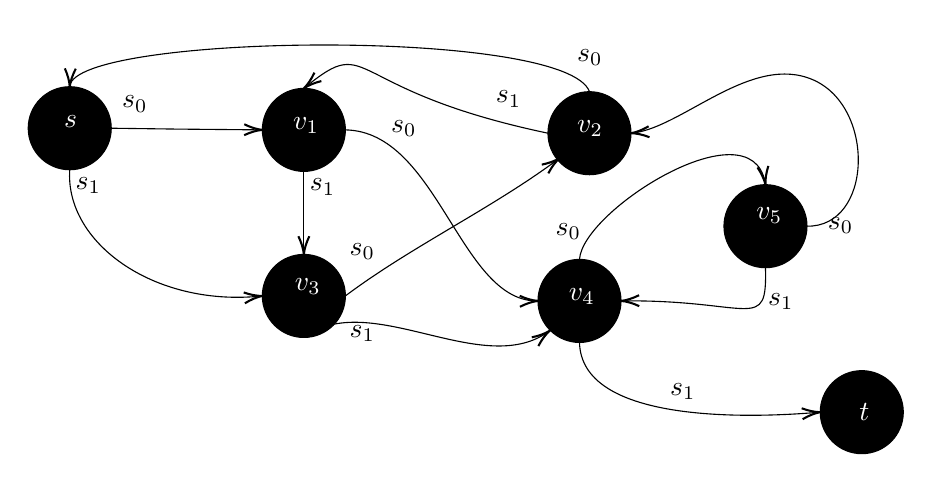
\begin{tikzpicture}[x=0.6pt,y=0.6pt,yscale=-1,xscale=1]
%uncomment if require: \path (0,300); %set diagram left start at 0, and has height of 300

%Shape: Circle [id:dp5495329281078569] 
\draw  [fill={rgb, 255:red, 0; green, 0; blue, 0 }  ,fill opacity=1 ] (32,49) .. controls (32,35.19) and (43.19,24) .. (57,24) .. controls (70.81,24) and (82,35.19) .. (82,49) .. controls (82,62.81) and (70.81,74) .. (57,74) .. controls (43.19,74) and (32,62.81) .. (32,49) -- cycle ;
%Straight Lines [id:da33331850965746734] 
\draw    (82,49) -- (121.98,49.53) -- (171,49.98) ;
\draw [shift={(173,50)}, rotate = 180.52] [color={rgb, 255:red, 0; green, 0; blue, 0 }  ][line width=0.75]    (10.93,-3.29) .. controls (6.95,-1.4) and (3.31,-0.3) .. (0,0) .. controls (3.31,0.3) and (6.95,1.4) .. (10.93,3.29)   ;
%Shape: Circle [id:dp8549825383964691] 
\draw  [fill={rgb, 255:red, 0; green, 0; blue, 0 }  ,fill opacity=1 ] (173,50) .. controls (173,36.19) and (184.19,25) .. (198,25) .. controls (211.81,25) and (223,36.19) .. (223,50) .. controls (223,63.81) and (211.81,75) .. (198,75) .. controls (184.19,75) and (173,63.81) .. (173,50) -- cycle ;
%Straight Lines [id:da15070581279870932] 
\draw    (198,75) -- (198,123) ;
\draw [shift={(198,125)}, rotate = 270] [color={rgb, 255:red, 0; green, 0; blue, 0 }  ][line width=0.75]    (10.93,-3.29) .. controls (6.95,-1.4) and (3.31,-0.3) .. (0,0) .. controls (3.31,0.3) and (6.95,1.4) .. (10.93,3.29)   ;
%Shape: Circle [id:dp4390825091110777] 
\draw  [fill={rgb, 255:red, 0; green, 0; blue, 0 }  ,fill opacity=1 ] (345,52) .. controls (345,38.19) and (356.19,27) .. (370,27) .. controls (383.81,27) and (395,38.19) .. (395,52) .. controls (395,65.81) and (383.81,77) .. (370,77) .. controls (356.19,77) and (345,65.81) .. (345,52) -- cycle ;
%Shape: Circle [id:dp9757305512769809] 
\draw  [fill={rgb, 255:red, 0; green, 0; blue, 0 }  ,fill opacity=1 ] (173,150) .. controls (173,136.19) and (184.19,125) .. (198,125) .. controls (211.81,125) and (223,136.19) .. (223,150) .. controls (223,163.81) and (211.81,175) .. (198,175) .. controls (184.19,175) and (173,163.81) .. (173,150) -- cycle ;
%Shape: Circle [id:dp6476109813645592] 
\draw  [fill={rgb, 255:red, 0; green, 0; blue, 0 }  ,fill opacity=1 ] (339,153) .. controls (339,139.19) and (350.19,128) .. (364,128) .. controls (377.81,128) and (389,139.19) .. (389,153) .. controls (389,166.81) and (377.81,178) .. (364,178) .. controls (350.19,178) and (339,166.81) .. (339,153) -- cycle ;
%Shape: Circle [id:dp9387189635111892] 
\draw  [fill={rgb, 255:red, 0; green, 0; blue, 0 }  ,fill opacity=1 ] (451,108) .. controls (451,94.19) and (462.19,83) .. (476,83) .. controls (489.81,83) and (501,94.19) .. (501,108) .. controls (501,121.81) and (489.81,133) .. (476,133) .. controls (462.19,133) and (451,121.81) .. (451,108) -- cycle ;
%Shape: Circle [id:dp6728900489022538] 
\draw  [fill={rgb, 255:red, 0; green, 0; blue, 0 }  ,fill opacity=1 ] (509,220) .. controls (509,206.19) and (520.19,195) .. (534,195) .. controls (547.81,195) and (559,206.19) .. (559,220) .. controls (559,233.81) and (547.81,245) .. (534,245) .. controls (520.19,245) and (509,233.81) .. (509,220) -- cycle ;
%Curve Lines [id:da06839655673782064] 
\draw    (223,50) .. controls (278.44,50.99) and (291.74,151.95) .. (337.6,153) ;
\draw [shift={(339,153)}, rotate = 178.78] [color={rgb, 255:red, 0; green, 0; blue, 0 }  ][line width=0.75]    (10.93,-3.29) .. controls (6.95,-1.4) and (3.31,-0.3) .. (0,0) .. controls (3.31,0.3) and (6.95,1.4) .. (10.93,3.29)   ;
%Curve Lines [id:da30024168681774177] 
\draw    (364,178) .. controls (364.99,225.52) and (461.05,224.04) .. (507.6,220.12) ;
\draw [shift={(509,220)}, rotate = 175.03] [color={rgb, 255:red, 0; green, 0; blue, 0 }  ][line width=0.75]    (10.93,-3.29) .. controls (6.95,-1.4) and (3.31,-0.3) .. (0,0) .. controls (3.31,0.3) and (6.95,1.4) .. (10.93,3.29)   ;
%Curve Lines [id:da031177664907863667] 
\draw    (370,27) .. controls (356.28,-11.22) and (69.81,-8.14) .. (57.41,22.11) ;
\draw [shift={(57,24)}, rotate = 271.79] [color={rgb, 255:red, 0; green, 0; blue, 0 }  ][line width=0.75]    (10.93,-3.29) .. controls (6.95,-1.4) and (3.31,-0.3) .. (0,0) .. controls (3.31,0.3) and (6.95,1.4) .. (10.93,3.29)   ;
%Curve Lines [id:da19551484489395188] 
\draw    (364,128) .. controls (365.79,98.44) and (466.95,34.79) .. (475.76,81.55) ;
\draw [shift={(476,83)}, rotate = 261.95] [color={rgb, 255:red, 0; green, 0; blue, 0 }  ][line width=0.75]    (10.93,-3.29) .. controls (6.95,-1.4) and (3.31,-0.3) .. (0,0) .. controls (3.31,0.3) and (6.95,1.4) .. (10.93,3.29)   ;
%Curve Lines [id:da5453571551089418] 
\draw    (345,52) .. controls (220.26,25.76) and (239.59,-8.8) .. (199.24,23.99) ;
\draw [shift={(198,25)}, rotate = 320.6] [color={rgb, 255:red, 0; green, 0; blue, 0 }  ][line width=0.75]    (10.93,-3.29) .. controls (6.95,-1.4) and (3.31,-0.3) .. (0,0) .. controls (3.31,0.3) and (6.95,1.4) .. (10.93,3.29)   ;
%Curve Lines [id:da7736997926226343] 
\draw    (223,150) .. controls (262.6,120.3) and (311.02,97.46) .. (350.8,67.9) ;
\draw [shift={(352,67)}, rotate = 143.13] [color={rgb, 255:red, 0; green, 0; blue, 0 }  ][line width=0.75]    (10.93,-3.29) .. controls (6.95,-1.4) and (3.31,-0.3) .. (0,0) .. controls (3.31,0.3) and (6.95,1.4) .. (10.93,3.29)   ;
%Curve Lines [id:da35489757719958615] 
\draw    (57,74) .. controls (54.03,117.56) and (106.93,156.22) .. (171.05,150.2) ;
\draw [shift={(173,150)}, rotate = 173.85] [color={rgb, 255:red, 0; green, 0; blue, 0 }  ][line width=0.75]    (10.93,-3.29) .. controls (6.95,-1.4) and (3.31,-0.3) .. (0,0) .. controls (3.31,0.3) and (6.95,1.4) .. (10.93,3.29)   ;
%Curve Lines [id:da7424500525745132] 
\draw    (198,175) .. controls (237.6,145.3) and (304.64,199.89) .. (344.79,171.87) ;
\draw [shift={(346,171)}, rotate = 143.13] [color={rgb, 255:red, 0; green, 0; blue, 0 }  ][line width=0.75]    (10.93,-3.29) .. controls (6.95,-1.4) and (3.31,-0.3) .. (0,0) .. controls (3.31,0.3) and (6.95,1.4) .. (10.93,3.29)   ;
%Curve Lines [id:da3132040250840804] 
\draw    (501,108) .. controls (540.44,108.6) and (542.5,36.73) .. (505,20) .. controls (468.25,3.6) and (426.87,47.76) .. (396.83,51.8) ;
\draw [shift={(395,52)}, rotate = 355.43] [color={rgb, 255:red, 0; green, 0; blue, 0 }  ][line width=0.75]    (10.93,-3.29) .. controls (6.95,-1.4) and (3.31,-0.3) .. (0,0) .. controls (3.31,0.3) and (6.95,1.4) .. (10.93,3.29)   ;
%Curve Lines [id:da9721751571878057] 
\draw    (476,133) .. controls (477,172.8) and (468.09,152.21) .. (390.18,152.99) ;
\draw [shift={(389,153)}, rotate = 359.27] [color={rgb, 255:red, 0; green, 0; blue, 0 }  ][line width=0.75]    (10.93,-3.29) .. controls (6.95,-1.4) and (3.31,-0.3) .. (0,0) .. controls (3.31,0.3) and (6.95,1.4) .. (10.93,3.29)   ;

% Text Node
\draw (87,28) node [anchor=north west][inner sep=0.75pt]   [align=left] {$\displaystyle s_{0}$};
% Text Node
\draw (52,40) node [anchor=north west][inner sep=0.75pt]  [color={rgb, 255:red, 255; green, 255; blue, 255 }  ,opacity=1 ] [align=left] {$\displaystyle s$};
% Text Node
\draw (59,77) node [anchor=north west][inner sep=0.75pt]   [align=left] {$\displaystyle s_{1}$};
% Text Node
\draw (249,43) node [anchor=north west][inner sep=0.75pt]   [align=left] {$\displaystyle s_{0}$};
% Text Node
\draw (190,41) node [anchor=north west][inner sep=0.75pt]  [color={rgb, 255:red, 255; green, 255; blue, 255 }  ,opacity=1 ] [align=left] {$\displaystyle v_{1}$};
% Text Node
\draw (200,78) node [anchor=north west][inner sep=0.75pt]   [align=left] {$\displaystyle s_{1}$};
% Text Node
\draw (361,0) node [anchor=north west][inner sep=0.75pt]   [align=left] {$\displaystyle s_{0}$};
% Text Node
\draw (361,43) node [anchor=north west][inner sep=0.75pt]  [color={rgb, 255:red, 255; green, 255; blue, 255 }  ,opacity=1 ] [align=left] {$\displaystyle v_{2}$};
% Text Node
\draw (224,117) node [anchor=north west][inner sep=0.75pt]   [align=left] {$\displaystyle s_{0}$};
% Text Node
\draw (191,138) node [anchor=north west][inner sep=0.75pt]  [color={rgb, 255:red, 255; green, 255; blue, 255 }  ,opacity=1 ] [align=left] {$\displaystyle v_{3}$};
% Text Node
\draw (224,166) node [anchor=north west][inner sep=0.75pt]   [align=left] {$\displaystyle s_{1}$};
% Text Node
\draw (348,105) node [anchor=north west][inner sep=0.75pt]   [align=left] {$\displaystyle s_{0}$};
% Text Node
\draw (356,144) node [anchor=north west][inner sep=0.75pt]  [color={rgb, 255:red, 255; green, 255; blue, 255 }  ,opacity=1 ] [align=left] {$\displaystyle v_{4}$};
% Text Node
\draw (417,201) node [anchor=north west][inner sep=0.75pt]   [align=left] {$\displaystyle s_{1}$};
% Text Node
\draw (512,101) node [anchor=north west][inner sep=0.75pt]   [align=left] {$\displaystyle s_{0}$};
% Text Node
\draw (469,95) node [anchor=north west][inner sep=0.75pt]  [color={rgb, 255:red, 255; green, 255; blue, 255 }  ,opacity=1 ] [align=left] {$\displaystyle v_{5}$};
% Text Node
\draw (476,147) node [anchor=north west][inner sep=0.75pt]   [align=left] {$\displaystyle s_{1}$};
% Text Node
\draw (531,213) node [anchor=north west][inner sep=0.75pt]  [color={rgb, 255:red, 255; green, 255; blue, 255 }  ,opacity=1 ] [align=left] {$\displaystyle t$};
% Text Node
\draw (312,25) node [anchor=north west][inner sep=0.75pt]   [align=left] {$\displaystyle s_{1}$};


\end{tikzpicture}

  \caption{An example instance of the arrival problem.}\label{arrivalDiagram}
\end{figure}
There is an obvious algorithm to solve the $\textsc{Arrival}$ problem;
just simulate the walk. However, the case of instances where $t$ is not reachable pose a problem.
If $t$ is not reachable, the walk must cycle infinitely and never terminate!
The following content demonstrates that this is a non issue.
\begin{definition}[Hopeful and Desperation]
  Let $(V, s, t, s_0, s_1)$ be an instance of the $\arr$ problem. A vertex $v \in V$
  is \emph{hopeful} if there is a path $v \to t$ in the directed graph defined with
  the vertex set $V$ the edge set $E \subseteq V \times V$ with $(u, v) \in E$ if and
  only if either $s_0(u) = v$ or $s_1(u) = v$. The \emph{desperation} of a hopeful vertex
  $v$ is the length of the shortest path from $v$ to $t$.
\end{definition}
\begin{lemma}[\citep{arrivalBasic}]
  Let $(V, s, t, s_0, s_1)$  be an instance of the $\arr$ problem. If $v \in V$ is hopeful,
  the arrival walk passes through $v$ at most $2^{|V|}$ times.
\end{lemma}
\begin{proof}
  Begin by noting that if a vertex is hopeful, it's desperation is at most $|V|$. I perform
  an induction on the desperation of $v$. Suppose the desperation of $v \in V$ is 1. Then either
  $s_0(v) = t$ or $s_1(v) = t$. If $s_0(v) = t$, $t$ will be reached after passing through $v$ once.
  If $s_1(v) = t$ and $s_0(v) \neq t$ $t$ will be reached after passing through $v$ twice. In
  both cases $v$ is passed through at most $2^1 = 2$ times. \\
  Suppose that all hopeful vertices with desperation $d - 1$ are passed through at most $2^{d-1}$ times.
  Then if $v \in V$ is hopeful with desperation $d$, for some hopeful $w \in V$ with desperation
  $d - 1$ either $s_0(v) = w$ or $s_1(v) = w$. So at least every second passing of $v$, the
  walk will proceed to $w$. But the walk can pass through $w$ at most $2^{d-1}$ times,
  so the walk can pass through $v$ at most $2 \cdot 2^{d - 1} = 2^d$ times.
\end{proof}
\begin{cor}\label{walkFinite}
  Let $(V, s, t, s_0, s_1)$ be an instance of the $\arr$ problem. Then the arrival
  walk either reaches $t$, or reaches a vertex which is not hopeful.
\end{cor}
From \cref{walkFinite} it is clear that deciding an instance of the $\arr$ problem is
equivalent to deciding whether or not the arrival walk reaches $t$ or reaches a vertex which
is not hopeful. 
\begin{definition}[Processed Arrival]
  Let $(V, s, t, s_0, s_1)$ be an instance of the arrival problem. Let
  $\sim$ be the equivalence relation on $V$ generated by $u \sim v$ if
  $u$ and $v$ are both not hopeful.
  The \emph{processed arrival problem}
  is a set of vertices $V' = V / \sim$, the canonical projections of $s, t, s_0, s_1$ into $V'$,
  and a choice of representative $\overline{t} \in V'$ of all the non hopeful vertices in $V$.
\end{definition}
The set of non hopeful vertices can be easily computed in linear time with a breadth first search
from $t$. From this point on I will therefore refer
to instances of the $\arr$ problem exclusively as tuples $(V, s, t, \overline{t}, s_0, s_1)$ 
constructed as above.
\begin{cor}[\citep{arrivalBasic}]
  Let $(V, s, t, \overline{t}, s_0, s_1)$ be an instance of the $\arr$ problem,
  and $n = |V|$. The time complexity of the $\arr$ problem is $O(n \cdot 2^n)$.
\end{cor}
\begin{proof}
  I reason that the arrival walk on the processed instance $(V, s, t, \overline{t}, s_0, s_1)$
  has it's walk length bounded by $O(n \cdot 2^n)$. Every vertex $v \in V$ with $v \neq \overline{t}$
  is hopeful with desperation at most $n$, so by \cref{walkFinite} can be passed through at most
  $2^{n}$ times. If the walk reaches $t$ or $\overline{t}$ it terminates, and there are at most
  $n$ vertices $w \in V$ such that $w \not\in \{t, \overline{t}\}$, so the walk can take at most
  $n \cdot 2^n$ steps.
\end{proof}
There are in fact instances of the $\arr$ problem with exponentially long walks. A diagram
of such a case can be seen in \cref{expLongArrival}.
\begin{figure}
  \caption{An arrival instance with an exponentially long walk.}\label{expLongArrival}
\end{figure}
\begin{definition}[Switching Flow]
  Let $(V, s, t, s_0, s_1)$ be an arrival graph. A \emph{switching flow} is a pair of maps 
  $f_0, f_1 : V \to V$ such that the following axioms hold.
  \begin{itemize}
    \item For all $v \in V$
  \end{itemize}
\end{definition}
Interestingly, the $\textsc{Arrival}$ problem is polynomial-time reducible to $\trsk$. 
This idea was used in \citep{gärtner2021subexponential} in a slightly different form to what is presented here
to give a sub-exponential time algorithm for solving the $\textsc{Arrival}$ problem. 
The rest of this section will be demonstrating the reduction from $\arr$ to $\trsk$.

\chapter{State of the art Algorithms} \label{stateAlgsChap}
\section{Overview}
Recent developments have been made in upper bounds for the $\trsk$ problem.
The critical component to the algorithmic improvements is
the surprising result from \citep{fasterTarski} that $\trsk(N, 3)$
can be solved in at most $O(\log^2 N)$ queries.
The idea is roughly as follows; suppose I have
a monotone function $f : [N]^3 \to [N]^3$ and an algorithm which
given a coordinate $i \in \{1, 2, 3\}$ and a value $v \in [N]$
returns a monotone point $x \in [N]^3$ with the guarantee
that $x_i = v$. If this algorithm takes $q(N)$ queries in the worst case,
then a fixpoint of $f$ can be found in $O(\log N \cdot q(N))$ in the
same fashion as \cref{dQiYiAlg}. This problem will prove to be
important, so I will define it in it's own right.
\newcommand{\trsks}{\textsc{Tarski*}}
\begin{definition}[\trsks]
  The problem $\trsks(N, d)$ is, given oracle access to a monotone function $f : [N]^d \to [N]^d$,
  a coordinate $i \in \{1, ..., d\}$, and value $v \in [N]$, find a monotone point $x \in [N]^d$ such that
  $x_i = v$. 
\end{definition}
The breakthrough in \citep{fasterTarski} was in detailing a so-called inner-algorithm which leads to
the following result.
\begin{theorem}[\citep{fasterTarski}]
  The query complexity of $\trsks(N, 3)$ is $O(\log N)$.
\end{theorem}
Fearnley et al. also gave a method of decomposition, allowing for $\trsk$ in higher
dimensions to be decomposed into a product of sorts of lower
dimensional problems. This can be seen as a generalization of the method in \cref{dQiYiAlg}.
Dang et al. solve $\trsk(N, d)$ by solving an instance $A$ of $\trsk(N, 1)$ in the $d$-th 
where every query of the monotone function from $\trsk(N, 1)$ at $v$ is answered by recursively finding
a fixpoint in the slice at the $d-th$ coordinate with value $v$. It then follows that
a soution to $A$ can be used to recover a solution of the entire problem. The algorithm of
Fearnley et al. shows that it is possible to make more general decompositions using a method
which I call \emph{fixpoint decomposition}. There is slight complication with making this precise
which will be detailed in a later section of this chapter.
\begin{theorem}[Fixpoint Decomposition, \citep{fasterTarski}]\label{fixDecomp}
  For positive integers $a, b \in \zpos$, given an algorithm $A$
  which can solve $\trsk(N, a)$ in $p(N, a)$ queries, and an algorithm $B$
  which can solve $\trsk(N, b)$ in $p(N, b)$ queries, the problem
  $\trsk(N, a + b)$ can be solved in $O(p(N, a)\cdot (q(N, b) + 2))$ queries.
\end{theorem}
Chen and Li take this one step further; instead of decomposing the $\trsk$ problem
they show that it is possible to make a decomposition on $\trsks$ using a method
I will call \emph{monotone decomposition}. The details
of this are more complicated still than \cref{fixDecomp}, and will be shared in a later
section.
\begin{theorem}[Monotone Decomposition, \citep{chenLi}]
  For positive integers $a, b \in \zpos$, given an algorithm $A$
  which can solve $\trsks(N, a)$ in $p(N, a)$ queries, and an algorithm $B$
  which an solve $\trsks(N, b)$ in $q(N, b)$ queries, the problem $\trsks(N, a + b)$
  can be solved in $O((b + 1) \cdot p(N, a) \cdot q(N, b))$ queries.
\end{theorem}

\section{The Inner Algorithm}
I will not detail the inner algorithm in it's entirety, nor prove it's correctness;
the reader is instead directed to \citep{fasterTarski}. Instead I will introduce
the main invariant, showing how the algorithm can make progress in the important 
cases. I require a weakening of the invariant used in \cref{dQiYiAlg}; whereas
in \cref{dQiYiAlg} two opposing monotone points are maintained essentially
defining the top and bottom of a sublattice on which the monotone function
naturally restricts, the inner algorithm allows for more possibilities.
\begin{definition}[Witness, \citep{fasterTarski}]
  Let $f : [N]^3 \to [N]^3$. A \emph{down set witness} is a pair of points
  $(d, b) \in ([N]^3)^2$ such that $f(d)_3 = f(b)_3$ and for some $i, j \in \{1, 2\}$
  with $i \neq j$,
  \begin{itemize}
    \item $d_i = b_i$, $b_j \leq d_j$, $f(b)_j \geq b_j$, and $f(d)_j \leq d_j$,
    \item $f(d)_3 \geq d_3$ and $f(b)_3 \geq b_3$.
  \end{itemize}
  An \emph{up set witness} is a pair of points
  $(a, u) \in ([N]^3)^2$ such that $f(a)_3 = f(u)_3$ and for some $i, j \in \{1, 2\}$
  with $i \neq j$,
  \begin{itemize}
    \item $a_i = u_i$, $a_j \leq u_j$, $f(a)_j \geq a_j$, and $f(u)_j \leq u_j$,
    \item $f(d)_3 \geq d_3$ and $f(b)_3 \geq b_3$.
  \end{itemize}
\end{definition}
[add ref to figure with witness diagrams] shows the different possible configurations
of witnesses to aid the reader in digesting this definition.
Now for the main invariant of the inner algorithm.
\begin{definition}[Inner algorithm invariant]
  Let $f : [N]^3 \to [N]^3$ be a monotone function. The \emph{inner algorithm invariant}
  is an up set witness $(d, b)$ and a down set witness $(a, u)$ such that $u \leq d$.
\end{definition}
\begin{prop}
  Let $f : [N]^3 \to [N]^3$ be a monotone function with $(a, u)$, $(d, b)$ up
  and down set witnesses respectively satisfying the inner algorithm invariant.
  Then there is a point $x \in [N]^3$ with $a \leq x \leq b$ and $f(x) = x$.
\end{prop}
\begin{proof}
  sorry
\end{proof}

\section{Fixpoint Decomposition}
Throughout I will fix $a, b \in \zpos$,
$d = a + b$, and $f : [N]^a \times [N]^b \to [N]^a \times [N]^b$.
Suppose I have an algorithm $A$ which can solve $\trsk(N, a)$,
and an algorithm $B$ which can solve $\trsk(N, b)$. A naive approach 
for finding a fixpoint of $f$ would be to define a
function on the right hand side of the lattice
$f_r : [N]^b \to [N]^b$ where given $x_r \in [N]^b$ the value of 
$f_r(x_r)$
is computed by defining the slice $f_l : [N]^a \to [N]^a$
such that $f_l(x_l) = f((x_l, x_r))$, finding a fixpoint $x_l^* \in [N]^a$
of $f_l$, then using $f(x_l^*, x_r)_{-l}$ as the result of $f_r(x_r)$.
The punch-line is then that if $x_r$ is a fixpoint of $f_r$, then if
$x_l^*$ was the fixpoint of $f_l$ associated with $x_r$ the point
$(x_l^*, x_r)$ is a fixpoint of $f$. This does not work however -
there is no guarantee that $f_r$ is monotone. That is,
if points $x_r, x_r' \in [N]^b$ are queried by algorithm $B$
with $x_r \leq x_r'$ it is not necessarily the case that the associated
fixpoints of $f_l$ $x_l^*$ and $x_l'^* \in [N]^a$ satisfy $x_l^* \leq x_l'^*$, so
monotonocity of $f$ does not carry over. The trick will thus be
to find a way to guarantee that $x_l*$ and $x_l'^*$ satisfy 
$x_l^* \leq x_l'^*$ whenever $x_r \leq x_r'$. Fortunately
this is achieveable; in \cref{fixDecompAlg} the issue is solved
by carefully choosing bounds of the sublattice to search in based
on previously computed points. The correctness of which will be
the concern of the remainder of this section.

\begin{algorithm}[h]
  \caption{\citep{fasterTarski}}\label{fixDecompAlg}
  \begin{algorithmic}[1]
    \Procedure{FixpointDecomposition}{\\
      \qquad monotone $f : [N]^a \times [N]^b \to [N]^a \times [N]^b$,\\
      \qquad algorithm $A$ for solving $\trsk(N, a)$, \\
      \qquad algorithm $B$ for solving $\trsk(N, b)$ 
    }
    \State $\text{prev} \subseteq [N]^a \times [N]^b \gets \emptyset$
    \Procedure{$f_r$}{$x_r \in [N]^b$}
      \Procedure{$f_l$}{$x_l \in [N]^a$}
        \Return $f((x_l, x_r))_{-r}$.
      \EndProcedure
      \State $\bot_l \gets \bigvee\{p_l : (p_l, p_r) \in \text{prev} : p_r \leq x_r \}$
      \State $\top_r \gets \bigwedge\{p_l : (p_l, p_r) \in \text{prev} : p_r \geq x_r \}$
      \State using algorithm $A$ find a fixpoint $x_l^*$ of $f_l$ in the sublattice with bounds
      $\bot_l$, $\top_l$.
      \State $\text{prev} \gets \text{prev} \cup \{(x_l^*, x_r)\}$
      \State \Return $f((x_l^*, x_r))_{-l}$.
    \EndProcedure
    \State run algorithm $B$ on $f_r$ to find fixpoint $x_r^*$
    \State \Return $(x_l^*, x_r^*)$ where $x_l^*$ is the fixpoint of $f_l$ 
    found when evaluating $f(x_r^*)$.
  \EndProcedure
  \end{algorithmic}
\end{algorithm}

\begin{lemma}\label{orderPreserved}
  If $(p_l, p_r), (p_l', p_r') \in \text{prev}$ with $p_r \leq p_r'$ then
  $p_l \leq p_l'$
\end{lemma}
\begin{proof}
  Suppose without loss of generality that $p_r$ was queried by algorithm $B$
  before $p_r'$. Then when $p_r'$ is queried, $p_l$ is an element of
  $\{pl : (pl, pr) \in \text{prev} : p_r \leq p_r'\}$ whence $\bot_l \geq p_l$,
  so the fixpoint found by algorithm $A$ satisfies $x_l^* \geq p_l$.
\end{proof}
\begin{lemma}
  At line 7 of \cref{fixDecompAlg} $\bot_l \leq \top_l$.
\end{lemma}
\begin{proof}
  By \cref{orderPreserved} I have for all 
  $p_l \in \{p_l : (p_l, p_r) \in \text{prev} : p_r \leq x_r \}$ and
  $p_l' \in \{p_l : (p_l, p_r) \in \text{prev} : p_r \geq x_r \}$ that
  $p_l \leq p_l'$. Then by definition of $\wedge$ and $\vee$ $\bot_l \leq \top_l$.
\end{proof}
\begin{lemma}\label{leftRestricts}
  At line 7 of \cref{fixDecompAlg} I have $f_l(\bot_l) \geq \bot_l$ and $f_r(\top_l) \leq \top_l$.
\end{lemma}
\begin{proof}
  I prove the first case and the second is similar. Suppose not. That is,
  for some $i \in [a]$ I have $f_l(\bot_l)_i < (\bot_l)_i$. If 
  $L = \{p_l : (p_l, p_r) \in \text{prev} : p_r \leq x_r \}$ is empty then
  $\vee L = \vec{1}$ and the claim holds. If $L$ is non-empty then by definition
  of finite joins, there is some $(p_l, p_r) \in \text{prev}$ such that $(p_l)_i = (\bot_l)_i$
  and $(p_l, p_r) \leq (x_l, x_r)$. But $f(((p_l, p_r))_{-r})_i = (p_l)_i$ so
  I contradict monotinicity.
\end{proof}
\begin{lemma}
  At line 7 of $\cref{fixDecompAlg}$ $f_l$ is a monotone function on the lattice
  $[N]^d_{\geq \bot_l, \leq \top_l}$.
\end{lemma}
\begin{proof}
  That $f_l$ is monotone follows from an inductive application of \cref{sliceMonotone}.
  Then the rest follows from \cref{leftRestricts} and \cref{restricts}.
\end{proof}
\begin{prop}
  The point $(x_l^*, x_r^*)$ returned by \cref{fixDecompAlg} is a fixpoint of $f$.
\end{prop}
\begin{proof}
  \cref{orderPreserved} guarantees that $f_r$ is monotone, and hence
  on line 10 a fixpoint $x_r^*$ can be found. Then by construction
  $(x_l^*, x_r^*)$ is clearly a fixpoint of $f$.
\end{proof}
\begin{proofOf}{\cref{fixDecomp}}
  Suppose algorithm $A$ takes at most $p(N, a)$ queries and algorithm $B$ takes at most
  $q(N, a)$ queries to find a fixpoint. Then every query of $f_r$ by algorithm $A$
  makes at most $q(N, b)$ queries to $f$ to find a fixpoint of $f_l$, so
  given algorithm $A$ makes a most $p(N, a)$ queries, the entire algorithms
  makes at most $p(N, a) \cdot q(N, b)$ queries to $f$.
\end{proofOf}


%todo all of this.
\section{Monotone Decomposition} \label{monotoneDecompChap}
The algorithm described in \cref{fixDecompChapter} makes a decomposition
of $\trsk$ by decomposing into smaller fixpoint computation problems, with
the asymptotic improvement coming from the fact that there is an algorithm
to efficently solve the $\trsk(N, 3)$ problem. We can do better however;
Chen and Li describe in \citep{chenLi} a method of decomposing the $\trsks$
problem instead. To save space, this section will show the algorithms used
but for proofs of correcteness the reader is referred to \citep{chenLi}.
It will be simpler to give an overview after a definition of 
an auxiliary problem.
\newcommand{\trskst}{\textsc{Tarksi}^*}
\begin{definition}[$\trskst$, \citep{chenLi}] \label{trskst}
  The problem $\trskst(N, d)$ is given oracle access to a function $f : [N]^d \to \{-1, 0, 1\}^d$
  such that,
  \begin{enumerate}
    \item for each $x \in [N]^d$ and $i \in [d]$, $x_i + f(x)_i \in [N]^d$,
    \item for each $x, y \in [N]^d$ with $x \leq y$, $(x, 0) + f(x) \leq (y, 0) + f(y)$,
  \end{enumerate}
  find a point $x \in [N]^d$ such that $f(x) \geq 0$ or $f(x) \leq 0$.
\end{definition}
This function $f$ is designed to be an indicator of a monotone function $F : [N]^d \to [N]^d$;
that is if I define $f$ coordinatewise as 
$f(x)_i = \begin{cases} 1, & F(x)_i > x_i \\ 0, & F(x)_i = x_i \\ -1, & F(x)_i < x_i \end{cases}$
then $f$ satisfies the conditions in \cref{trskst}. The first condition is the requirement that
the codomain of $F$ is correct, and the second is monotonicity. It is also clear that $\trsks(N, d)$ 
trivially reduces to $\trskst(N, d)$. Chen and Li then wish to make decompositions from
$\trskst(N, a + b)$ into $\trskst(N, a)$ and $\trskst(N, b)$. The fixpoint decomposition
method \cref{fixDecompAlg} does not obviously apply here; it is not clear what to do with the extra
coordinate in the codomain, and further if I split into $f_l$ and $f_r$ similarly to \cref{fixDecompAlg},
if $(x_l, x_r) \in [N]^a \times [N]^b$, are found as monotone points of $f_l$ and $f_r$,
$x_l$ can be a monotone-down point, and $x_r$ a monotone up point so $(x_l, x_r)$ is not necessarily
a monotone point of $f$. Chen and Li's first step towards a solution is defining a refinement of the
$\trskst$ problem.
\begin{definition}[$\textsc{RefinedTarski}^*$, \citep{chenLi}]
  Given a function $f : [N]^d \to \{-1, 0, 1\}^{d + 1}$ as in \cref{trskst}, find
  a pair of points $\bot, \top \in [N]^d$ such that $\bot \leq \top$, for each $i \in [d]$,
  $f(\bot)_i \geq 0$, $f(\top)_i \leq 0$, and at least one of the following hold,
  \begin{enumerate}
    \item $f(\bot)_{d + 1} = 1$,
    \item $f(\top)_{d + 1} = -1$,
    \item $f(\bot) = f(\top) = 0$.
  \end{enumerate}
\end{definition}
Interestingly, Chen and Li show that this problem is no harder than $\trskst$ in the sense
that it can be solved in at most two queries to a $\trskst$ orcacle. Their algorithm for doing this is
shown in \cref{refinedTarskAlg}.
\begin{algorithm}[H]
  \caption{\citep{chenLi}. An auxiliary algorithm for monotone decomposition.} \label{refinedTarskAlg}
  \begin{algorithmic}[1]
    \Procedure{RefinedTarski$^*$}{\\
      \qquad $f : [N]^d \to \{-1, 0, 1\}^{d + 1}$ as in \cref{trskst},\\
      \qquad algorithm $A$ for solving $\trskst(N, d)$
    }
    \State $(\bot, \top) \gets (\vec{1}, \vec{N})$
    \State Let $g^+ : [N]^d \to [N]^{d+1}$ with $g^+(x)_i = 
      \begin{cases} 1, & i = d + 1 \text{ and } g(x)_{d + 1} \geq 0 \\ g(x)_i, & \text{otherwise}\end{cases}$
    \State $x \gets A(g^+)$ with bounds $\bot$, $\top$
    \State \If{$g^+(x) = -1$} $\top \gets x$ and \Return $(\bot, \top)$ \EndIf
    \State $\bot \gets x$
  \State Let $g^- : [N]^d \to [N]^{d+1}$ with $g^+(x)_i = 
    \begin{cases} -1, & i = d + 1 \text{ and } g(x)_{d + 1} \leq 0 \\ g(x)_i, & \text{otherwise}\end{cases}$
    \State $y \gets A(g^-)$ with bounds $\bot$, $\top$
    \If{$g^-(y)_{d + 1} = 1$} $\bot \gets y$ \algorithmicelse\ $\top \gets y$ \EndIf
    \State \Return $(\bot, \top)$
  \EndProcedure
  \end{algorithmic}
\end{algorithm}
Correctness is relatively simple to verify and is ommitted for brevity. Note
$g^+$ and $g^-$ also need to be verified to satisfy \cref{trskst}.
Now for the main algorithm in \cref{monDecompAlg}.
\begin{algorithm}[h]
  \caption{\citep{chenLi}. An algorithm for decomposing monotone point computation problems.} \label{monDecompAlg}
  \begin{algorithmic}[1]
    \Procedure{MonotoneDecomposition}{\\
      \qquad $f : [N]^{a + b}  \to \{-1, 0, 1\}^{a + b + 1}$ as in \cref{trskst},\\
      \qquad algorithm $A$ for solving $\trsk(N, a)$, \\
      \qquad algorithm $B$ for solving $\trsk(N, b)$ 
    }
    \State $\mathrm{prev} \gets \emptyset$
    \Procedure{$f_r : [N]^b \to \{-1, 0, 1\}^{b + 1}$}{$x_r \in [N]^b$}
      \State $\bot_l \gets \bigvee\{p_l : (p_l, p_r) \in \mathrm{prev}, \; p_r \leq x_r \}$
      \State $\top_l \gets \bigwedge\{p_l : (p_l, p_r) \in \mathrm{prev}, \; p_r \geq x_r \}$
      \For{$j$ from $a + 1$ to $a + b + 1$ }
      \Procedure{$f_l^j : [N]^a \to \{-1, 0, 1\}^{a + 1}$}{$x_l \in [N]^a$}
        \State $y \gets f((x_l, x_r))$
        \State \Return $(y_1, ..., y_a, y_j)$.
      \EndProcedure
      \State $(\bot_l^j, \top_l^j) \gets \Call{RefinedTarski$^*$}{f_l^j, A}$ with bounds $\bot_l$, $\top_l$
      \State $(\bot_l, \top_l) \gets (\bot_l^j, \top_l^j)$
      \EndFor

      \State $\mathrm{prev} \gets \mathrm{prev} \cup \{(\bot_l, x_r)\}$
      \State $x \gets f((\bot_l, x_r))$
      \State \Return $f(x_{a + 1}, ..., x_{b + 1})$.
    \EndProcedure
    \State $x_r^* \gets B(f_r)$
    \State let $(\bot_l, \top_l)$ be the bounds found when evaluating $f_r(x_r^*)$
    \If{$f_r(x_r^*) \geq 0$} \Return $(\bot_l, x_r^*)$ \algorithmicelse\ \Return $(\top_l, x_r^*)$ \EndIf
  \EndProcedure
  \end{algorithmic}
\end{algorithm}
\begin{lemma}
  \cref{monDecompAlg} gives a correct solution to $\trskst$.
\end{lemma}
\begin{sproof}
The proof that all intermediate functions restrict to the transient bounds $(\bot_l, \top_l)$ is similar
to the proof of correctness of \cref{fixDecompAlg} with a few extra cases. 
  The crux of the proof for \cref{monDecompAlg} 
is \citep[Lemma 6]{chenLi}
where it is shown that at line 16, for each $i \in \{a + 1, ..., b + 1\}$, and every $p, p' \in [\bot_l, \top_l]$,
  $f((p, x_r^*))_i = f((p', x_r^*))_i$. This is because inductively from the loop on line 6 I find
$\bot_l \geq \bot_l^i$ and $\top_l \leq \top_l^i$,
  so if $f((\bot_l, x_r^*))_i = 1$, then since $(\bot_l^i, \top_l^i)$ was a solution to
  $\textsc{RefinedTarski}^*(f_l^i, A)$ I find $f((p, x_r^*)) \geq f((\bot_l, x_r^*))_i \geq f_l^i(\bot_l^i)_i = 1$.
  The cases with $f((\bot_l, x_r^*))_i \in \{-1, 0 \}$ are similar. \\
  When the algorithm returns on line 17, $(\bot_l, \top_l)$ was a solution to
  $\textsc{RefinedTarski}^*$ in the slice at $x_r^*$, so for each $i \in [a]$, 
  $f((\bot_l, x_r^*))_i \geq 0$ and $f((\top_l, x_r^*))_i \leq 0$, so the condition on line 17
  ensures that the returned point is a solution to $\trskst$.
\end{sproof}
For complete proof of correctness of \cref{monDecompAlg} see \citep{chenLi}. It is clear that
\cref{monDecompAlg} gives the asymptotic bound in \cref{monDecomp}.

\section{Open Problems}
Many problems on the algorithmic complexity of $\trsk$ remain 
open. The most impressive upper bound on query complexity would be the following.
\begin{open} \label{tarskiInP}
  Is the query complexity of $\trsk(N, d)$ $O(\poly(\log N) \cdot \poly(d))$?
\end{open}
The implications of a result in the positive for \cref{tarskiInP} would be significant to say the least.
For example, it would give a polynomial time algorithm for
computing the exact value of simple stochastic games as described in \cref{ssgs},
which has remained an open problem since 1992 when studied by Condon in \citep{condon}.
It would also imply a polynomial-time algorithm for the $\arr$ problem as described in \cref{arr},
the complexity of which has seen a significant amount of study in recent years
\citep{gärtner2021subexponential, gärtner2018arrival, arrivalBasic, arrLowerBound}.
Another implication would be a polynomial time algorithm for approximating the value of
stochastic games as in \cref{shapleyChap}. The strength of the implications of \cref{tarskiInP}
are evidence that solving it in the near future is unlikely, and that considering weaker conjectures
might be more realistic.
\begin{open} \label{tarskiFixedParameterTractable}
  Is the query complexity of 
  $\trsk(N, d)$ $O(\log^2 N)$ for fixed $d$? That is, is $\trsk$ fixed-parameter tractable?
\end{open}
Recent results such as \cref{tightThreeDimension} from \citep{fasterTarski} make this seem
plausible. Perhaps the notion of a 'witness' as described in \cref{witnessDef} can be
generalized to higher dimensions, with a method of halfing the search space as in \cref{innerMainCase}
in a potentially exponential number of queries? A useful intermediate result towards this problem could be
the following.
\begin{open} \label{tightFourDimension}
  Is the query complexity of $\trsk(N, 4)$ $O(\log^2 N)$?
\end{open}
Improved lower bounds for the $\trsk$ problem would also be an interesting
result. A first step could be the following.
\begin{open}
  For some $d \in \Z_{> 2}$ is the query complexity of
  $\trsk(N, d)$ $\omega(\log^2 N)$?
\end{open}



\chapter{Related Problems} \label{relatedProblemsChapter}
In this chapter, I discuss three problems problems in algorithmic game theory
which are polynomial-time reducible to $\trsk$; $\arr$, simple stochastic games, and
shapley's stochastic games, with the goal of motivating study on the $\trsk$ problem.
\section{The Arrival Problem}
\newcommand{\flowin}{\ensuremath{f_{\text{in}}}}
\newcommand{\glowin}{\ensuremath{g_{\text{in}}}}

The arrival problem is, given a directed graph with
a particular structure and designated source and target vertex,
decide whether or not a particular walk starting at the source
ever reaches the target. In \citep{gärtner2021subexponential} a sub-exponential
time algorithm for arrival is developed which reduces the problem to $\trsk$ of some form.
It turns out that $\arr$ is in fact polynomial time reducible to $\trsk$.
While this is not explicity stated in \citep{gärtner2021subexponential}, essentially
all of the theory for this reduction is included so credit goes to them. In this section,
I give the basic definitions of the $\arr$ problem as well as a complete proof
of polynomial time reduction from $\arr$ to $\trsk$.
\begin{definition}[Arrival Graph]
  An \emph{arrival graph} is a set of vertices $V$, a pair of
  vertices $s, t \in V$, and a pair of maps 
  $s_0, s_1 : V \to V$. 
\end{definition}
\begin{definition}[Arrival Walk]
  Let $(V, s, t, s_0, s_1)$ be an arrival graph. The \emph{arrival walk}
  on this graph is a sequence of vertices $(v_i)_{i \in \znn} \in V$
  such that $v_0 = s$, and $v_{i+1} = 
  \begin{cases} 
    s_0(v_i), & \text{$n_i$ even}\\  
    s_1(v_i), & \text{$n_i$ odd},
  \end{cases}$
  where $n_i$ is the number of times $v_i$ has appeared previously in
  the sequence.
\end{definition}
 A diagram of an example arrival graph is shown in 
in $\cref{arrivalDiagram}$.
It is clear that the arrival walk for a particular arrival graph
is entirely defined by the structure of the graph, which is what
lead it to be called a zero player graph game in \citep{arrivalBasic}.
\begin{definition}[$\textsc{Arrival}$]
  The $\textsc{Arrival}$ problem is, given an arrival graph $(V, s, t, s_0, s_1)$,
  decide whether or not the arrival walk ever reaches $t$.
\end{definition}
\begin{figure}[h]
  \centering
  \tikzset{every picture/.style={line width=0.75pt}} %set default line width to 0.75pt        

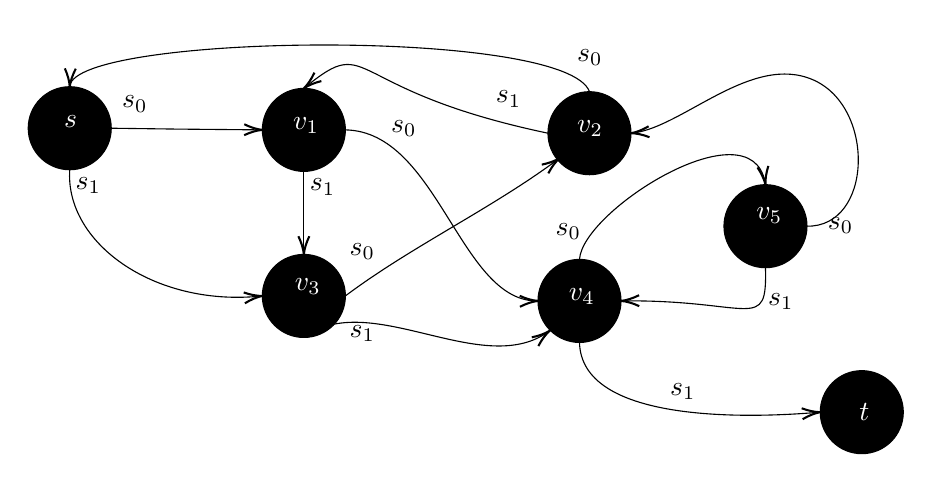
\begin{tikzpicture}[x=0.6pt,y=0.6pt,yscale=-1,xscale=1]
%uncomment if require: \path (0,300); %set diagram left start at 0, and has height of 300

%Shape: Circle [id:dp5495329281078569] 
\draw  [fill={rgb, 255:red, 0; green, 0; blue, 0 }  ,fill opacity=1 ] (32,49) .. controls (32,35.19) and (43.19,24) .. (57,24) .. controls (70.81,24) and (82,35.19) .. (82,49) .. controls (82,62.81) and (70.81,74) .. (57,74) .. controls (43.19,74) and (32,62.81) .. (32,49) -- cycle ;
%Straight Lines [id:da33331850965746734] 
\draw    (82,49) -- (121.98,49.53) -- (171,49.98) ;
\draw [shift={(173,50)}, rotate = 180.52] [color={rgb, 255:red, 0; green, 0; blue, 0 }  ][line width=0.75]    (10.93,-3.29) .. controls (6.95,-1.4) and (3.31,-0.3) .. (0,0) .. controls (3.31,0.3) and (6.95,1.4) .. (10.93,3.29)   ;
%Shape: Circle [id:dp8549825383964691] 
\draw  [fill={rgb, 255:red, 0; green, 0; blue, 0 }  ,fill opacity=1 ] (173,50) .. controls (173,36.19) and (184.19,25) .. (198,25) .. controls (211.81,25) and (223,36.19) .. (223,50) .. controls (223,63.81) and (211.81,75) .. (198,75) .. controls (184.19,75) and (173,63.81) .. (173,50) -- cycle ;
%Straight Lines [id:da15070581279870932] 
\draw    (198,75) -- (198,123) ;
\draw [shift={(198,125)}, rotate = 270] [color={rgb, 255:red, 0; green, 0; blue, 0 }  ][line width=0.75]    (10.93,-3.29) .. controls (6.95,-1.4) and (3.31,-0.3) .. (0,0) .. controls (3.31,0.3) and (6.95,1.4) .. (10.93,3.29)   ;
%Shape: Circle [id:dp4390825091110777] 
\draw  [fill={rgb, 255:red, 0; green, 0; blue, 0 }  ,fill opacity=1 ] (345,52) .. controls (345,38.19) and (356.19,27) .. (370,27) .. controls (383.81,27) and (395,38.19) .. (395,52) .. controls (395,65.81) and (383.81,77) .. (370,77) .. controls (356.19,77) and (345,65.81) .. (345,52) -- cycle ;
%Shape: Circle [id:dp9757305512769809] 
\draw  [fill={rgb, 255:red, 0; green, 0; blue, 0 }  ,fill opacity=1 ] (173,150) .. controls (173,136.19) and (184.19,125) .. (198,125) .. controls (211.81,125) and (223,136.19) .. (223,150) .. controls (223,163.81) and (211.81,175) .. (198,175) .. controls (184.19,175) and (173,163.81) .. (173,150) -- cycle ;
%Shape: Circle [id:dp6476109813645592] 
\draw  [fill={rgb, 255:red, 0; green, 0; blue, 0 }  ,fill opacity=1 ] (339,153) .. controls (339,139.19) and (350.19,128) .. (364,128) .. controls (377.81,128) and (389,139.19) .. (389,153) .. controls (389,166.81) and (377.81,178) .. (364,178) .. controls (350.19,178) and (339,166.81) .. (339,153) -- cycle ;
%Shape: Circle [id:dp9387189635111892] 
\draw  [fill={rgb, 255:red, 0; green, 0; blue, 0 }  ,fill opacity=1 ] (451,108) .. controls (451,94.19) and (462.19,83) .. (476,83) .. controls (489.81,83) and (501,94.19) .. (501,108) .. controls (501,121.81) and (489.81,133) .. (476,133) .. controls (462.19,133) and (451,121.81) .. (451,108) -- cycle ;
%Shape: Circle [id:dp6728900489022538] 
\draw  [fill={rgb, 255:red, 0; green, 0; blue, 0 }  ,fill opacity=1 ] (509,220) .. controls (509,206.19) and (520.19,195) .. (534,195) .. controls (547.81,195) and (559,206.19) .. (559,220) .. controls (559,233.81) and (547.81,245) .. (534,245) .. controls (520.19,245) and (509,233.81) .. (509,220) -- cycle ;
%Curve Lines [id:da06839655673782064] 
\draw    (223,50) .. controls (278.44,50.99) and (291.74,151.95) .. (337.6,153) ;
\draw [shift={(339,153)}, rotate = 178.78] [color={rgb, 255:red, 0; green, 0; blue, 0 }  ][line width=0.75]    (10.93,-3.29) .. controls (6.95,-1.4) and (3.31,-0.3) .. (0,0) .. controls (3.31,0.3) and (6.95,1.4) .. (10.93,3.29)   ;
%Curve Lines [id:da30024168681774177] 
\draw    (364,178) .. controls (364.99,225.52) and (461.05,224.04) .. (507.6,220.12) ;
\draw [shift={(509,220)}, rotate = 175.03] [color={rgb, 255:red, 0; green, 0; blue, 0 }  ][line width=0.75]    (10.93,-3.29) .. controls (6.95,-1.4) and (3.31,-0.3) .. (0,0) .. controls (3.31,0.3) and (6.95,1.4) .. (10.93,3.29)   ;
%Curve Lines [id:da031177664907863667] 
\draw    (370,27) .. controls (356.28,-11.22) and (69.81,-8.14) .. (57.41,22.11) ;
\draw [shift={(57,24)}, rotate = 271.79] [color={rgb, 255:red, 0; green, 0; blue, 0 }  ][line width=0.75]    (10.93,-3.29) .. controls (6.95,-1.4) and (3.31,-0.3) .. (0,0) .. controls (3.31,0.3) and (6.95,1.4) .. (10.93,3.29)   ;
%Curve Lines [id:da19551484489395188] 
\draw    (364,128) .. controls (365.79,98.44) and (466.95,34.79) .. (475.76,81.55) ;
\draw [shift={(476,83)}, rotate = 261.95] [color={rgb, 255:red, 0; green, 0; blue, 0 }  ][line width=0.75]    (10.93,-3.29) .. controls (6.95,-1.4) and (3.31,-0.3) .. (0,0) .. controls (3.31,0.3) and (6.95,1.4) .. (10.93,3.29)   ;
%Curve Lines [id:da5453571551089418] 
\draw    (345,52) .. controls (220.26,25.76) and (239.59,-8.8) .. (199.24,23.99) ;
\draw [shift={(198,25)}, rotate = 320.6] [color={rgb, 255:red, 0; green, 0; blue, 0 }  ][line width=0.75]    (10.93,-3.29) .. controls (6.95,-1.4) and (3.31,-0.3) .. (0,0) .. controls (3.31,0.3) and (6.95,1.4) .. (10.93,3.29)   ;
%Curve Lines [id:da7736997926226343] 
\draw    (223,150) .. controls (262.6,120.3) and (311.02,97.46) .. (350.8,67.9) ;
\draw [shift={(352,67)}, rotate = 143.13] [color={rgb, 255:red, 0; green, 0; blue, 0 }  ][line width=0.75]    (10.93,-3.29) .. controls (6.95,-1.4) and (3.31,-0.3) .. (0,0) .. controls (3.31,0.3) and (6.95,1.4) .. (10.93,3.29)   ;
%Curve Lines [id:da35489757719958615] 
\draw    (57,74) .. controls (54.03,117.56) and (106.93,156.22) .. (171.05,150.2) ;
\draw [shift={(173,150)}, rotate = 173.85] [color={rgb, 255:red, 0; green, 0; blue, 0 }  ][line width=0.75]    (10.93,-3.29) .. controls (6.95,-1.4) and (3.31,-0.3) .. (0,0) .. controls (3.31,0.3) and (6.95,1.4) .. (10.93,3.29)   ;
%Curve Lines [id:da7424500525745132] 
\draw    (198,175) .. controls (237.6,145.3) and (304.64,199.89) .. (344.79,171.87) ;
\draw [shift={(346,171)}, rotate = 143.13] [color={rgb, 255:red, 0; green, 0; blue, 0 }  ][line width=0.75]    (10.93,-3.29) .. controls (6.95,-1.4) and (3.31,-0.3) .. (0,0) .. controls (3.31,0.3) and (6.95,1.4) .. (10.93,3.29)   ;
%Curve Lines [id:da3132040250840804] 
\draw    (501,108) .. controls (540.44,108.6) and (542.5,36.73) .. (505,20) .. controls (468.25,3.6) and (426.87,47.76) .. (396.83,51.8) ;
\draw [shift={(395,52)}, rotate = 355.43] [color={rgb, 255:red, 0; green, 0; blue, 0 }  ][line width=0.75]    (10.93,-3.29) .. controls (6.95,-1.4) and (3.31,-0.3) .. (0,0) .. controls (3.31,0.3) and (6.95,1.4) .. (10.93,3.29)   ;
%Curve Lines [id:da9721751571878057] 
\draw    (476,133) .. controls (477,172.8) and (468.09,152.21) .. (390.18,152.99) ;
\draw [shift={(389,153)}, rotate = 359.27] [color={rgb, 255:red, 0; green, 0; blue, 0 }  ][line width=0.75]    (10.93,-3.29) .. controls (6.95,-1.4) and (3.31,-0.3) .. (0,0) .. controls (3.31,0.3) and (6.95,1.4) .. (10.93,3.29)   ;

% Text Node
\draw (87,28) node [anchor=north west][inner sep=0.75pt]   [align=left] {$\displaystyle s_{0}$};
% Text Node
\draw (52,40) node [anchor=north west][inner sep=0.75pt]  [color={rgb, 255:red, 255; green, 255; blue, 255 }  ,opacity=1 ] [align=left] {$\displaystyle s$};
% Text Node
\draw (59,77) node [anchor=north west][inner sep=0.75pt]   [align=left] {$\displaystyle s_{1}$};
% Text Node
\draw (249,43) node [anchor=north west][inner sep=0.75pt]   [align=left] {$\displaystyle s_{0}$};
% Text Node
\draw (190,41) node [anchor=north west][inner sep=0.75pt]  [color={rgb, 255:red, 255; green, 255; blue, 255 }  ,opacity=1 ] [align=left] {$\displaystyle v_{1}$};
% Text Node
\draw (200,78) node [anchor=north west][inner sep=0.75pt]   [align=left] {$\displaystyle s_{1}$};
% Text Node
\draw (361,0) node [anchor=north west][inner sep=0.75pt]   [align=left] {$\displaystyle s_{0}$};
% Text Node
\draw (361,43) node [anchor=north west][inner sep=0.75pt]  [color={rgb, 255:red, 255; green, 255; blue, 255 }  ,opacity=1 ] [align=left] {$\displaystyle v_{2}$};
% Text Node
\draw (224,117) node [anchor=north west][inner sep=0.75pt]   [align=left] {$\displaystyle s_{0}$};
% Text Node
\draw (191,138) node [anchor=north west][inner sep=0.75pt]  [color={rgb, 255:red, 255; green, 255; blue, 255 }  ,opacity=1 ] [align=left] {$\displaystyle v_{3}$};
% Text Node
\draw (224,166) node [anchor=north west][inner sep=0.75pt]   [align=left] {$\displaystyle s_{1}$};
% Text Node
\draw (348,105) node [anchor=north west][inner sep=0.75pt]   [align=left] {$\displaystyle s_{0}$};
% Text Node
\draw (356,144) node [anchor=north west][inner sep=0.75pt]  [color={rgb, 255:red, 255; green, 255; blue, 255 }  ,opacity=1 ] [align=left] {$\displaystyle v_{4}$};
% Text Node
\draw (417,201) node [anchor=north west][inner sep=0.75pt]   [align=left] {$\displaystyle s_{1}$};
% Text Node
\draw (512,101) node [anchor=north west][inner sep=0.75pt]   [align=left] {$\displaystyle s_{0}$};
% Text Node
\draw (469,95) node [anchor=north west][inner sep=0.75pt]  [color={rgb, 255:red, 255; green, 255; blue, 255 }  ,opacity=1 ] [align=left] {$\displaystyle v_{5}$};
% Text Node
\draw (476,147) node [anchor=north west][inner sep=0.75pt]   [align=left] {$\displaystyle s_{1}$};
% Text Node
\draw (531,213) node [anchor=north west][inner sep=0.75pt]  [color={rgb, 255:red, 255; green, 255; blue, 255 }  ,opacity=1 ] [align=left] {$\displaystyle t$};
% Text Node
\draw (312,25) node [anchor=north west][inner sep=0.75pt]   [align=left] {$\displaystyle s_{1}$};


\end{tikzpicture}

  \caption{The goal of the arrival problem is to decide whether a partiular walk on a directed graph with a particular
  structure reaches the target. On successive visits to a particular
  vertex the outgoing edge taken alternates. In this example
  the walk begins $s \to v_1 \to v_4 \to s \to v_3 \to \ldots$.} \label{arrivalDiagram}
\end{figure}
There is an obvious algorithm to solve the $\textsc{Arrival}$ problem;
just simulate the walk. Cases of instances where $t$ is not reachable pose a problem however -
the walk must cycle infinitely and never terminate!
The following content demonstrates that this is a non issue.
\begin{definition}[Hopeful and Desperation]
  Let $(V, s, t, s_0, s_1)$ be an instance of the $\arr$ problem. A vertex $v \in V$
  is \emph{hopeful} if there is a path $v \to t$ in the directed graph defined with
  the vertex set $V$ and edge set $E \subseteq V \times V$ with $(u, v) \in E$ if and
  only if either $s_0(u) = v$ or $s_1(u) = v$. The \emph{desperation} of a hopeful vertex
  $v$ is the length of the shortest path from $v$ to $t$.
\end{definition}
\begin{lemma}[\citep{arrivalBasic}]
  Let $(V, s, t, s_0, s_1)$  be an instance of the $\arr$ problem. If $v \in V$ is hopeful,
  the arrival walk passes through $v$ at most $2^{|V|}$ times.
\end{lemma}
\begin{proof}
  Begin by noting that if a vertex is hopeful, it's desperation is at most $|V|$. I perform
  an induction on the desperation of $v$. Suppose the desperation of $v \in V$ is 1. Then either
  $s_0(v) = t$ or $s_1(v) = t$. If $s_0(v) = t$, $t$ will be reached after passing through $v$ once.
  If $s_1(v) = t$ and $s_0(v) \neq t$ $t$ will be reached after passing through $v$ twice. In
  both cases $v$ is passed through at most $2^1 = 2$ times. \\
  Suppose that all hopeful vertices with desperation $d - 1$ are passed through at most $2^{d-1}$ times.
  Then if $v \in V$ is hopeful with desperation $d$, for some hopeful $w \in V$ with desperation
  $d - 1$ either $s_0(v) = w$ or $s_1(v) = w$. So at least every second passing of $v$, the
  walk will proceed to $w$. But the walk can pass through $w$ at most $2^{d-1}$ times,
  so the walk can pass through $v$ at most $2 \cdot 2^{d - 1} = 2^d$ times.
\end{proof}
\begin{cor}\label{walkFinite}
  Let $(V, s, t, s_0, s_1)$ be an instance of the $\arr$ problem. Then the arrival
  walk either reaches $t$, or reaches a vertex which is not hopeful.
\end{cor}
From \cref{walkFinite} it is clear that deciding an instance of the $\arr$ problem is
equivalent to deciding whether or not the arrival walk reaches $t$ or reaches a vertex which
is not hopeful.
\begin{definition}[Processed Arrival]
  Let $(V, s, t, s_0, s_1)$ be an instance of the arrival problem. It
  is without loss of generality to assume that the set of unhopeful vertices
  is non-empty. Let
  $\sim$ be the equivalence relation on $V$ generated by $u \sim v$ if
  $u$ and $v$ are both not hopeful.
  The \emph{processed arrival problem}
  is a set of vertices $V' = V / \sim$, the canonical projections of $s, t, s_0, s_1$ into $V'$,
  and a choice of representative $\overline{t} \in V'$ of all the non hopeful vertices in $V$.
\end{definition}
\begin{figure}[ht]
  \centering
  \tikzset{every picture/.style={line width=0.75pt}} %set default line width to 0.75pt        
  \raisebox{-0.5\height}{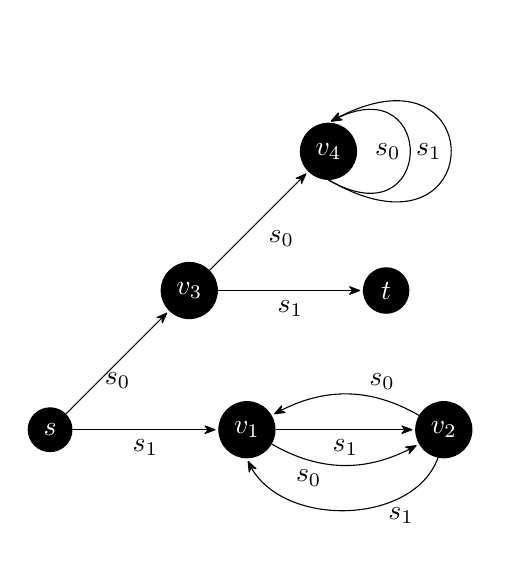
\begin{tikzpicture}[x=0.6pt,y=0.6pt,yscale=-1,xscale=1, 
  main/.style = {draw, circle, 
  fill={rgb, 255:red, 0; green, 0; blue, 0 }},
  text=white,
  node distance=2.5cm,
  ->,
  >={Stealth[round,sep]}]
  \node[main] (s) {$s$};
  \node[main] (1) [right of=s]{$v_1$};
  \node[main] (2) [right of=1]{$v_2$};
  \node[main] (3) [above right of=s]{$v_3$};
  \node[main] (4) [above right of=3]{$v_4$};
  
  % \node[main] (4) [right of=3]{$v_n$};
  \node[main] (t)[right of=3]{$t$};
  \draw (s) -- (3) node[midway, below, text=black]{$s_0$};
  \draw (s) -- (1) node[midway, below, text=black]{$s_1$};
  \draw (1) -- (2) node[midway, below, text=black]{$s_1$};
  \draw (3) -- (t) node[midway, below, text=black]{$s_1$};
  \draw (3) -- (4) node[midway, below right, text=black]{$s_0$};
  \draw (2) edge[bend left] node[near start, above, text=black]{$s_0$} (1);
  \draw (1) edge[bend left] node[near start, below, text=black]{$s_0$}(2);

  \draw (4.south) to[bend left=120, min distance=1.6cm] node[midway, left, text=black]{$s_0$} (4.north);
  \draw (4.south) to[bend left=120, min distance=2.4cm] node[midway, left, text=black]{$s_1$} (4.north);
  % \draw (4) edge[bend left] node[near start, above, text=black]{$s_0$}(1);
  \draw (2) edge[bend right=70, min distance=0.8cm] node[near start, below, text=black]{$s_1$} (1.south);
\end{tikzpicture}
}
  \hfil
  $\mapsto$
  \hfil
  \raisebox{-0.5\height}{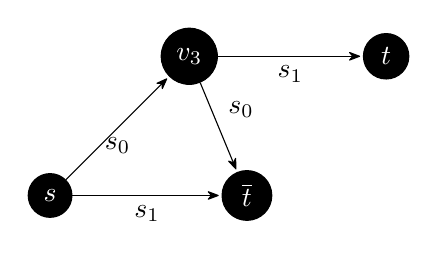
\begin{tikzpicture}[x=0.6pt,y=0.6pt,yscale=-1,xscale=1, 
  main/.style = {draw, circle, 
  fill={rgb, 255:red, 0; green, 0; blue, 0 }},
  text=white,
  node distance=2.5cm,
  ->,
  >={Stealth[round,sep]}]
  \node[main] (s) {$s$};
  \node[main] (1) [right of=s]{$\overline{t}$};
  \node[main] (3) [above right of=s]{$v_3$};
  
  % \node[main] (4) [right of=3]{$v_n$};
  \node[main] (4)[right of=3]{$t$};
  \draw (s) -- (3) node[midway, below, text=black]{$s_0$};
  \draw (s) -- (1) node[midway, below, text=black]{$s_1$};
  \draw (3) -- (4) node[midway, below, text=black]{$s_1$};
  \draw (3) -- (1) node[midway, above right, text=black]{$s_0$};
\end{tikzpicture}
}
  \caption{Instances of the arrival problem can be preprocessed so that every non-target vertex
  has a directed path to the target. An extra 'bad target' $\overline{t}$ is added which represents
  all the vertices with no directed path to the target $t$, and the problem becomes to decide
  which of the two targets is reached. From \cref{walkFinite} 
  the walk in the resultant graph must be finite.}\label{arrivalPreprocess}
\end{figure}
Noting that the set of non hopeful vertices can be easily computed in linear time with a breadth first search
from $t$, from this point on I will refer
to instances of the $\arr$ problem exclusively as tuples $(V, s, t, \overline{t}, s_0, s_1)$ 
constructed as above.
\begin{cor}[\citep{arrivalBasic}]
  The time complexity of the $\arr$ problem is $O(n \cdot 2^n)$.
\end{cor}
\begin{proof}
  I reason that the arrival walk on the processed instance $(V, s, t, \overline{t}, s_0, s_1)$
  has it's walk length bounded by $O(n \cdot 2^n)$. Every vertex $v \in V$ with $v \neq \overline{t}$
  is hopeful with desperation at most $n$, so by \cref{walkFinite} can be passed through at most
  $2^{n}$ times. If the walk reaches $t$ or $\overline{t}$ it terminates, and there are at most
  $n$ vertices $w \in V$ such that $w \not\in \{t, \overline{t}\}$, so the walk can take at most
  $n \cdot 2^n$ steps.
\end{proof}
There are in fact instances of the $\arr$ problem with exponentially long walks -
as seen in \cref{expLongArrival} - implying that the worst-case runtime of this algorithm is exponential.
Recently a sub-exponential\footnote{Specifically an algorithm running
in time $O(2^{\sqrt{n}})$.} upper bound for $\arr$ was given in \citep{gärtner2021subexponential}.
Interestingly, their algorithm involves a reduction from $\arr$ to $\trsk$. I will not detail
the reduction used in the sub-exponential algorithm, but will spend the remainder of the section
demonstrating a similar, yet simpler reduction from $\arr$ to $\trsk$.
\begin{figure}[h]
  \centering
  \tikzset{every picture/.style={line width=0.75pt}} %set default line width to 0.75pt        

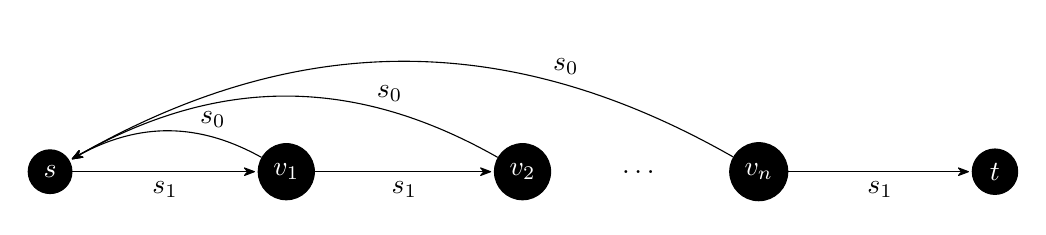
\begin{tikzpicture}[x=0.6pt,y=0.6pt,yscale=-1,xscale=1, 
  main/.style = {draw, circle, 
  fill={rgb, 255:red, 0; green, 0; blue, 0 }},
  text=white,
  node distance=3cm,
  ->,
  >={Stealth[round,sep]}]
  \node[main] (1) {$s$};
  \node[main] (2) [right of=1]{$v_1$};
  \node[main] (3) [right of=2]{$v_2$};
  \node[main] (4) [right of=3]{$v_n$};
  \node[main] (5)[right of=4]{$t$};
  \node[text=black] at ($(3)!.5!(4)$) {\ldots};
  \draw (1) -- (2) node[midway, below, text=black]{$s_1$};
  \draw (2) -- (3) node[midway, below, text=black]{$s_1$};
  \draw (4) -- (5) node[midway, below, text=black]{$s_1$};
  % \path (1) edge[loop above] node {$s_0$} (1);
  \draw (2) edge[bend left] node[near start, above, text=black]{$s_0$} (1);
  \draw (3) edge[bend left] node[near start, above, text=black]{$s_0$}(1);
  \draw (4) edge[bend left] node[near start, above, text=black]{$s_0$}(1);
\end{tikzpicture}

  \caption{There are instances of the arrival problem with exponentially long walks. An induction
  on the number of steps to get from $s \to v_i$ shows that walk on the above
  takes at least $\Omega(2^n)$ steps to reach $t$.}\label{expLongArrival}
\end{figure}
\begin{definition}[Switching Flow]
  Let $(V, s, t, \overline{t}, s_0, s_1)$ be an arrival graph. A \emph{switching flow} is a pair of maps 
  $f_0, f_1 : V \setminus \{t, \overline{t}\} \to \znn$ such that the following axioms hold.
    Let $\flowin(v) =
        \sum_{\substack{w \in V \\ s_0(w) = v}} f_0(w) 
        + \sum_{\substack{w \in V \\ s_1(w) = v}} f_1(w)$. 
  \begin{itemize}
    \item For all $v \in V \setminus \{s, t, \overline{t}\}$, $\flowin(v) = f_0(v) + f_1(v)$ (flow conservation),
    \item $\flowin(s) = f_0(s) + f_1(s) - 1$ (source flow conservation),
    \item For all $v \in V$, $f_1(v) \leq f_0(v) \leq f_1(v) + 1$ (switching).
  \end{itemize}
\end{definition}
\begin{notation}
    Throughout this section if $(f_0, f_1)$ are switching flows the notation $\flowin(v) =
        \sum_{\substack{w \in V \\ s_0(w) = v}} f_0(w) 
        + \sum_{\substack{w \in V \\ s_1(w) = v}} f_1(w)$ will be used. 
\end{notation}
  It was observed in \citep{arrivalBasic} that the walk on an arrival graph can be characterized
  by a switching flow.
  \begin{lemma}[\citep{arrivalBasic}]\label{walkSwitching}
    Let $(V, s, t, \overline{t}, s_0, s_1)$ be an instance of the $\arr$ problem. Define
    $f_0 : V \setminus \{t, \overline{t}\} \to \znn$ by $f_0(v) =$ the number of times $s_0(v)$
    is traversed in the arrival walk, and define $f_1$ similarly. Then $(f_0, f_1)$ is a switching
    flow.
  \end{lemma}
  \begin{proof}
    Flow conservation and source flow conservation follow from the fact that the walk must walk
    out of a vertex if it walks in, minus the initial step it takes from the source. Switching
    follows from the nature of the walk taking the $s_0$ edge on even passes, and $s_1$ edge on odd
    passes.
  \end{proof}
  I next establish a correspondence from arrival instances to monotone functions.
  \begin{definition}[Arrival Monotone Function]
    Let $(V, s, t, \overline{t}, s_0, s_1)$ be an instance of the arrival problem,
    $d = |V \setminus \{t, \overline{t}\}|$ and
    $(v_i)_{i \in [d]}$ be an enumeration of the vertices in 
    $V \setminus \{t, \overline{t}\}$. The \emph{arrival monotone function} is a function
    $f : \znn^d \to \znn^d$ defined coordinatewise as,
  \begin{align*}
    f((a_1, ..., a_d))_i = \begin{cases}
    \sum_{\substack{j \in [d] \\ s_0(v_j) = v_i}} \left\lceil \frac{a_j}{2} \right\rceil
      + \sum_{\substack{j \in [d] \\ s_1(v_j) = v_i}} \left\lfloor \frac{a_j}{2} \right\rfloor
      & v_i \neq s \\
    1 + \sum_{\substack{j \in [d] \\ s_0(v_j) = v_i}} \left\lceil \frac{a_j}{2} \right\rceil
      + \sum_{\substack{j \in [d] \\ s_1(v_j) = v_i}} \left\lfloor \frac{a_j}{2} \right\rfloor
      & v_i = s.
    \end{cases}
  \end{align*}
  \end{definition}
  \begin{lemma}\label{arrMonotoneIsMonotone}
    The arrival monotone function is monotone.
  \end{lemma}
  \begin{proof}
    Clearly the sum of monotone functions is also monotone, $\lceil \cdot \rceil$ and $\lfloor \cdot \rfloor$
    are monotone, composition of monotone functions is monotone, linear functions with non-negative coefficients
    are monotone, and constant functions are monotone. This encompasses all components of the above function,
    which is therefore montone.
  \end{proof}
  The monotone function was constructed precisely so that the following proposition holds.
  \begin{prop}\label{fixpointIsFlow}
    Let $f : \znn^d \to \znn^d$ be an arrival monotone function, and $a = (a_1, ..., a_d) \in \znn^d$. 
    Define $g_0(v_i) = \lceil \frac{a_i}{2} \rceil$ and $g_1(v_i) = \lfloor \frac{a_i}{2} \rfloor$. 
    Then $(g_0, g_1)$ is a switching flow if and only if $f(a) = a$.
  \end{prop}
  \begin{proof}
    $(\impliedby)$ For flow conservation, let $v_i \in V \setminus \{s, t, \overline{t}\}$. Then,
    \begin{align*}
      \sum_{\substack{j \in [d] \\ s_0(v_j) = v_i}} g_0(v_j) 
      + \sum_{\substack{j \in [d] \\ s_0(v_j) = v_i}} g_1(v_j) &= 
      \sum_{\substack{j \in [d] \\ s_0(v_j) = v_i}}  \left\lceil \frac{a_j}{2} \right\rceil
      + \sum_{\substack{j \in [d] \\ s_0(v_j) = v_i}} \left\lfloor \frac{a_j}{2} \right\rfloor \\
      &= f(a)_i \\ 
      &= a_i \\ 
      &= \left\lceil \frac{a_i}{2}\right\rceil + \left\lfloor \frac{a_i}{2}\right\rfloor \\
      &= g_0(v_i) + g_1(v_1).
    \end{align*}
    Source flow conservation follows similarly. Switching is clear from the definition of $\lfloor \cdot \rfloor$
    and $\lceil \cdot \rceil$. \\
    $(\implies)$ Let $g_0(v_i) = \left\lceil \frac{a_i}{2} \right\rceil$, 
    $g_1(v_i) = \left\lfloor \frac{a_i}{2} \right\rfloor$, and $(g_0, g_1)$ be a switching flow. Then
    for each $i \in [d]$ if $v_i \neq s$,
    \begin{align*}
      f((a_1, ..., a_d))_i &= 
    \sum_{\substack{j \in [d] \\ s_0(v_j) = v_i}} \left\lceil \frac{a_j}{2} \right\rceil
      + \sum_{\substack{j \in [d] \\ s_1(v_j) = v_i}} \left\lfloor \frac{a_j}{2} \right\rfloor \\
      &= \sum_{\substack{j \in [d] \\ s_0(v_j) = v_i}}  g_0(v_j) 
      + \sum_{\substack{j \in [d] \\ s_1(v_j) = v_i}}  g_1(v_j) \\
      &= g_0(v_i) + g_1(v_i) \qquad \text{(by flow conservation)} \\
      &= \left\lceil \frac{a_i}{2} \right\rceil + \left\lfloor \frac{a_i}{2} \right\rfloor = a_i,
    \end{align*}
    and if $v_i = s$,
    \begin{align*}
      f((a_1, ..., a_d))_i &= 
    1 + \sum_{\substack{j \in [d] \\ s_0(v_j) = v_i}} \left\lceil \frac{a_j}{2} \right\rceil
      + \sum_{\substack{j \in [d] \\ s_1(v_j) = v_i}} \left\lfloor \frac{a_j}{2} \right\rfloor \\
      &= 1 + \sum_{\substack{j \in [d] \\ s_0(v_j) = v_i}}  g_0(v_j) 
      + \sum_{\substack{j \in [d] \\ s_1(v_j) = v_i}}  g_1(v_j) \\
      &= 1 + g_0(v_i) + g_1(v_i) - 1 \qquad \text{(by source flow conservation)} \\
      &= \left\lceil \frac{a_i}{2} \right\rceil + \left\lfloor \frac{a_i}{2} \right\rfloor = a_i.
    \end{align*}
  \end{proof}
  The next proposition draws an intriguing connection between the arrival walk and monotone function.
  \newcommand{\lc}{\left\lceil}
  \newcommand{\rc}{\right\rceil}
  \newcommand{\lf}{\left\lfloor}
  \newcommand{\rf}{\right\rfloor}
  \begin{prop}\label{kleeneTarskiIsWalk}
    Let $(V, s, t, \overline{t}, s_0, s_1)$ be an instance of the problem, and $f$ be the 
    arrival monotone function. For $a \in \znn^d$ let $g_0(a) = \lc \frac{a}{2} \rc$ and 
    $g_1(a) = \lf \frac{a}{2} \rf$. For $i \in \{x \in \znn | x < n \}$ where $n$ number of steps
    to reach $t$ or $\overline{t}$, let 
    $(h_0^i : [d] \to \znn, h_1a^i : [d] \to \znn)_{i \in \znn}$
    be a sequence defined by $h_0^i(j) = $ the number of times the $s_0$ edge has been taken from $v_j$
    after $i$ steps in the walk, and define $h_1^i(j)$ similarly for the $s_1$ edge. Then for each $j \in [d]$
    $g_0(f^i(\vec{0}))_j = h_0^i(j)$ and $g_1(f^i(\vec{0}))_j = h_1^i(j)$.
  \end{prop}
  \begin{proof}
    By induction. For the base case where $i = 0$ no edges have been crossed, so for each
    $j \in [d]$ $h_0^i(j) = h_1^i(j) = 0 = \frac{f^0(\vec{0})_i}{2} = 0$. \\
    So suppose for some $i \in \znn$ the statement is true for all $j \in [i-1]$.
    Let $v_k \in V \setminus \{t, \overline{t}\}$ be the vertex the walk is at after $i - 1$ steps, and $v_l$ after $i-2$ steps.
    Then by the inductive hypothesis $f^{i-2}(\vec{0})_l + 1 = f^{i-1}(\vec{0})_l$ and for each
    $m \in [d] \setminus \{l\}$, $f^{i-2}(\vec{0})_m = f^{i-1}(\vec{0})_m$. It follows that
    $f^{i - 1}(\vec{0})_k + 1 = f^{i}(\vec{0})_k$, and the switching property of the monotone function
    guarantees that the extra unit appears on the correct edge.
  \end{proof}
  All of that is really just to say that in the case of monotone functions from the arrival problem,
  \emph{iteration from the bottom of the lattice as in \cref{kleeneTarski} is the walk}. This connection gives
  me some useful corollaries.
  \begin{cor}\label{walkLfp}
    Let $f$ be an arrival monotone function, 
    $(g_0, g_1)$ be the switching flow corresponding to an arrival walk as in \cref{walkSwitching},
    and $a \in \znn^d$ be the fixpoint corresponding to this switching flow as in \cref{fixpointIsFlow}.
    Then $a$ is the least fixpoint of $f$.
  \end{cor}
  \begin{proof}
    Using a similar argument to \cref{kleeneLfp}, iteration from the bottom of the lattice gives the least
    fixpoint. But \cref{kleeneTarskiIsWalk} says that iteration from the bottom of the lattice is the walk
    and will give the fixpoint corresponding to the switching flow of the walk.
  \end{proof}
  \begin{cor}
    Let $f : \znn^d \to \znn^d$ be an arrival monotone function, and $a \in \znn^d$ be a point
    such that $f(a) = a$. If 
    $f_{\text{in}} (t) = \sum_{\substack{i \in [d] \\ s_0(v_i) = t}}  \lc \frac{a_i}{2} \rc +
    \sum_{\substack{i \in [d] \\ s_1(v_i) = t}}  \lf \frac{a_i}{2} \rf$ and
    $\flowin(\overline{t}) = \sum_{\substack{i \in [d] \\ s_0(v_i) = \overline{t}}}  \lc \frac{a_i}{2} \rc +
    \sum_{\substack{i \in [d] \\ s_1(v_i) = \overline{t}}}  \lf \frac{a_i}{2} \rf$ are the inflows at $t$ and $\overline{t}$
    respectively. Exactly one of the following hold,
    \begin{itemize}
      \item $\flowin (t) = 1$ and $\flowin (\overline{t}) = 0$,
      \item $\flowin (t) = 0$ and $\flowin (\overline{t}) = 1$.
    \end{itemize}
  \end{cor}
  \begin{proof}
    The walk only terminates when it reaches either $t$ or $\overline{t}$, so the switching flow corresponding
    to the walk must satisfy exactly one of $\flowin(t) = 1$ and $\flowin(\overline{t}) = 0$ or 
    $\flowin(t) = 0$ and $\flowin(\overline{t}) = 1$. By \cref{walkLfp} the walk corresponds
    to the least fixpoint, and for all other switching flows $(g_0, g_1)$, at least one of $\glowin (t) \geq 1$ or
    $\glowin (\overline{t}) \geq 1$. Suppose for a contradiction that $\glowin (t) + \glowin (\overline{t}) \geq 2$ and let
    $a \in \znn^d$ be the point corresponding to $(g_0, g_1)$. Then
    $\sum_{i \in [d]} f(a)_i \leq \sum_{i \in [d]} a_i - 1$. But this contradicts $a$ being a fixpoint due to
    \cref{fixpointIsFlow}, from which I find $\glowin (t) + \glowin (\overline{t}) = 1$, and the claim follows.
  \end{proof}
  Remarkably, this implies that \emph{any} switching flow is certificate to the walk reaching either $t$
  or $\overline{t}$. Further, fixpoints are switching flows so deciding the $\arr$ problem is reducible
  to finding a fixpoint of a particular monotone function! I'm not quite finished yet however;
  the monotone functions of arrival instances considered so far have been on the infinite lattice $\znn^d$, but
  the $\trsk$ problem I defined is on the finite lattice $[N]^d$. This will turn out to not be an issue.
  \begin{notation}
    For $N \in \znn$ notation $[N]_0$ represents $[N] \cup \{0\}$.
  \end{notation}
  \newcommand{\no}{[N]_0}
  \begin{definition}[Bounded arrival monotone function]
    Let $(V, s, t, \overline{t}, s_0, s_1)$ be an instance of the arrival problem and $f$
    be it's corresponding arrival function. Let $n = |V|$ and $N = 2^n$. The \emph{bounded arrival monotone function}
    is a function $F : \no^d \to \no^d$ defined coordinatewise as $F(a)_i = \min(f(a)_i, N)$. 
  \end{definition}
  \begin{lemma}
    Let $F$ be a bounded arrival monotone function. Then $F$ is monotone.
  \end{lemma}
  \begin{proof}
    Similarly to the proof of \cref{arrMonotoneIsMonotone}, $\min(\cdot, \; N)$ is clearly monotone.
    Monotonicity then follows monotonicity of the arrival monotone function, and monotonicity
    being preserved under composition.
  \end{proof}
  \begin{lemma}\label{upOne}
    Let $f : \znn^d \to \znn^d$ be a monotone arrival function. If $a \in \znn^d$ then
    $\sum_{i \in [d]} f(a)_i \leq 1 + \sum_{i \in [d]} a_i$.
  \end{lemma}
  \begin{proof}
    I have 
    \begin{align*}
      \sum_{i \in [d]} f_i ((a_1, ..., a_d)) &= \sum_{i \in [d]} \begin{cases}
    \sum_{\substack{j \in [d] \\ s_0(v_j) = v_i}} \left\lceil \frac{a_j}{2} \right\rceil
      + \sum_{\substack{j \in [d] \\ s_1(v_j) = v_i}} \left\lfloor \frac{a_j}{2} \right\rfloor
      & v_i \neq s \\
    1 + \sum_{\substack{j \in [d] \\ s_0(v_j) = v_i}} \left\lceil \frac{a_j}{2} \right\rceil
      + \sum_{\substack{j \in [d] \\ s_1(v_j) = v_i}} \left\lfloor \frac{a_j}{2} \right\rfloor
      & v_i = s 
    \end{cases}\\
        &= 1 + \sum_{i \in [d]} \sum_{\substack{j \in [d] \\ s_0(v_j) = v_i}}  \left\lceil \frac{a_j}{2} \right\rceil
      + \sum_{i \in [d]} \sum_{\substack{j \in [d] \\ s_1(v_j) = v_i}} \left\lfloor \frac{a_j}{2} \right\rfloor. \\
    \end{align*}
    By construction of $s_0$ and $s_1$, for each $j \in [d]$ there is at most one
    $i \in [d]$ such that $s_0(v_j) = v_i$ and at most one $i' \in [d]$ such that $s_1(v_j) = v_{i'}$.
    So,
    \begin{align*}
        1 + \sum_{i \in [d]} \sum_{\substack{j \in [d] \\ s_0(v_j) = v_i}}  \left\lceil \frac{a_j}{2} \right\rceil
      + \sum_{i \in [d]} \sum_{\substack{j \in [d] \\ s_1(v_j) = v_i}} \left\lfloor \frac{a_j}{2} \right\rfloor
      &\leq 1 + \sum_{j \in [d]} \left\lceil \frac{a_j}{2} \right\rceil + \sum_{j \in [d]} \left\lfloor \frac{a_j}{2} \right\rfloor \\
      &= 1 + \sum_{i \in [d]} a_i. 
    \end{align*}
  \end{proof}
  \begin{lemma}[\citep{gärtner2021subexponential}]
    Let $(V, s, t, \overline{t}, s_0, s_1)$ be an instance of the arrival problem, 
    $n = |V|$, $N = 2^n$, $d = |V \setminus \{t, \overline{t}\}|$, 
    $f : \znn^d \to \znn^d$ be the arrival monotone function, and $F : \no^d \to \no^d$
    be the bounded arrival monotone function.
    If $a \in \no^d$ satisfies $F(a) = a$, then $f(a) = a$. 
  \end{lemma}
  \begin{proof}
    Begin by noting that for all $a \in \no^d$, $f(a) \geq F(a)$. Suppose for a contradiction that $f(a) \neq F(a)$.
    Then $F(a) > f(a)$. From \cref{upOne} combined with the fact that $F(a) = a$, I find that 
    $\sum_{i \in [d]} f(a)_i = 1 + \sum_{i \in [d]} a_i$. 
    It must therefore be the case that for some $i \in [d]$, $f(a)_j = 
    \begin{cases} a_j + 1 & j = i \\ a_j & j \neq i. \end{cases}$. By definition $F(a)_i = \min(f(a)_i, N)$
      from which it follows $a_i = N$ and $f(a)_i = N + 1$.
    For $\sum_{i \in [d]} f(a)_i = 1 + \sum_{i \in [d]} a_i$ I require that $f_{\text{in}}(t) = 0$ and $f_{\text{in}}(\overline{t}) = 0$.
    But \cref{walkFinite} combined with $a_i = N = 2^n$ implies that the walk must have terminated. That is,
    either $f_{\text{in}}(t) > 0$ or $f_{\text{in}}(\overline{t}) > 0$, which is a contradiction. 
  \end{proof}
  \begin{theorem}
    $\arr$ is polynomial time reducible to $\trsk$.
  \end{theorem}

\section{Simple Stochastic Games}\label{ssgs}
Simple stochastic games, as defined in \citep{condon}, are a class of
zero-sum games played on graphs with two players called the maximizer and minimizer
respectively. For the purposes of this dissertation I will consider only $\beta$-stopping
simple stochastic games which roughly speaking are simple stochastic games
where at every stage the game automatically halts with probability $\beta$.
Condon shows in \citep{condon} that these games necessarily have a rational value for rationally described instances
of the problem, and further that
the value can be achieved in pure stationary strategies which is to say
that players can achieve optimal expected payoff by fixing a deterministic
action for every one of their vertices prior to play commencing.
The relationship to $\trsk$ then comes from \citep{lowerBound}, where Etessami et al. show
that computing the \emph{exact} value of (not necessarily $\beta$-stopping) simple stochastic games as well as a pure stationary strategy profile
to achieve this value is 
polynomial-time reducible to $\trsk$. This section will lay out the required definitions,
and describe the aforementioned reduction to $\trsk$ in the special case of 
$\beta$-stopping simple stochastic games.

\newcommand{\vmax}{V_{\max}}
\newcommand{\vmin}{V_{\min}}
\begin{definition}[$\beta$-stopping Simple Stochastic Game]
  A \emph{$\beta$-stopping simple stochastic game} is a directed graph $G = (V, V_p, \vmax, \vmin, E, v_0, t, \beta)$ with designated start vertex $v_0 \in V$,
  target vertex $t \in V$, $\beta \in (0, 1] \cap \Q$,
  a partition of $V \setminus \{t\}$ into three disjoint subsets $V_p, V_{\min}, V_{\max}$,
  and a mapping $p : V_p \times V \to [0, 1] \cap \Q$
  such that for all $v_p \in V_p$,
  $v \in V$ if $(v_p, v) \not\in E$ I have $p(v_p, v) = 0$, for each
  $v_p \in V_p$ $\sum_{v \in V} p(v_p, v) = 1$, and for every $v \in V \setminus \{t\}$ there
  is necessarily an edge $(v, w) \in E$ for some $w \in V$. A \emph{play} in a simple stochastic game
  transpires as follows. A token is placed on the initial vertex of the game $v_0$.
  Let $v_i$ be the vertex on which the token currently lies. Then at each step, the game halts with probability $\beta$. If it did not halt and $v_i \in \vmax \; (\vmin)$
  then the maximizer (minimzer) chooses and edge $(v_i, v_{i + 1}) \in E$ for some $v_{i + 1} \in V$. If
  $v_i \in V_p$ then an edge $(v_i, w) \in E$ is chosen randomly with probability $p(v_i, w)$. If $v_i = t$
  then the game halts. 
  When the game halts, the maximizer gets a payoff of $1$ if the game reached
  $t$, and $0$ otherwise. The payoff of the minimizer is the negative of the maximizer's.
\end{definition}

\begin{figure}[h]
  \centering
  \tikzset{every picture/.style={line width=0.75pt}} %set default line width to 0.75pt        
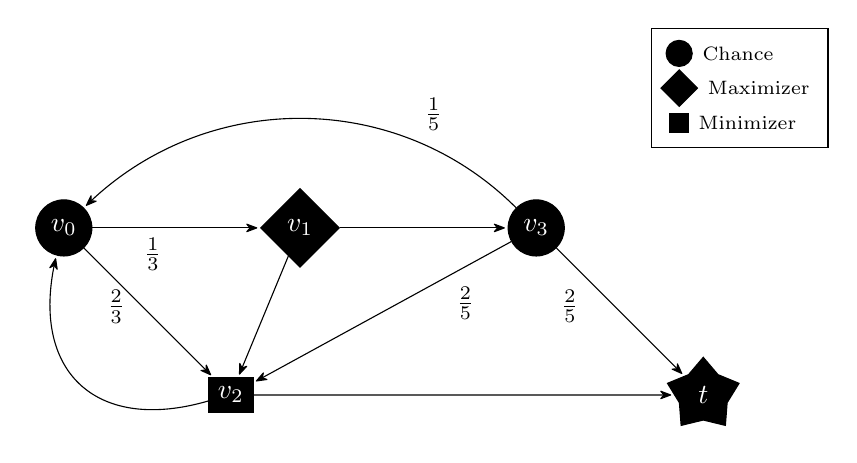
\begin{tikzpicture}[x=0.6pt,y=0.6pt,yscale=-1,xscale=1,
  main/.style = {draw, circle, 
  fill={rgb, 255:red, 0; green, 0; blue, 0 }, text=white},
  node distance=3cm,
  ->,
  >={Stealth[round,sep]},
  legend/.style={draw, circle,
  fill={rgb, 255:red, 0; green, 0; blue, 0 },
  text=black
  }
  ]

  \node[main] (v0) {$v_0$};
  \node[main, shape=diamond] (v1) [right of=v0] {$v_1$};
  \node[main, shape=rectangle] (v2) [below right of=v0] {$v_2$};
  \node[main] (v3) [right of=v1] {$v_3$};
  \node[main, shape=star] (t) [below right of=v3] {$t$};

  \draw (v0) -- (v1) node[near start, below right, text=black]{$\frac{1}{3}$};
  \draw (v0) -- (v2) node[near start, below, text=black]{$\frac{2}{3}$};

  \draw (v3) -- (t) node[near start, below left, text=black]{$\frac{2}{5}$};
  \draw (v3) -- (v2) node[near start, below right, text=black]{$\frac{2}{5}$};
  \draw (v3) to[bend left=45, min distance=1cm] node[near start, above right, text=black]{$\frac{1}{5}$} (v0);

  \draw (v1) -- (v3);
  \draw (v1) -- (v2); 

  \draw (v2) edge[bend right=60, min distance=1.5cm] (v0);
  \draw (v2) -- (t);

  \matrix [draw] at (current bounding box.north east) {
    \node[legend, label=right:\scriptsize Chance] {}; \\
    \node[legend, shape=diamond,label=right:\scriptsize Maximizer] {}; \\
    \node[legend, shape=rectangle,label=right:\scriptsize Minimizer] {}; \\
  };

\end{tikzpicture}

  \caption{In $\beta$-stopping simple stochastic games, one of the two players aims to maximize the probability
  of play reaching the target $t$, while the other aims to minimize it.}
\end{figure}

It is clear that since $\beta > 0$ the game eventually halts with probability $1$. 
\begin{definition}[Pure Stationary Strategy]
  Let $G = (V, V_p, \vmax, \vmin, E, v_0, t)$ be a simple stochastic game. A \emph{pure stationary strategy}
  for the maximizer is a mapping $\sigma : \vmax \to V$ with the requirement that for all $v \in \vmax$
  $(v, \sigma(v)) \in E$. The set of all such pure stationary strategies for the maximizer is denoted
  $S$. A pure stationary strategy for the minimizer is a map $\tau : \vmin \to V$ such that
  for all $v \in \vmin$ 
  $(v, \tau(v)) \in E$. The set of all such pure stationary strategies for the minimizer is denoted $T$. 
  A \emph{pure stationary strategy profile} is a pair $(\sigma, \tau) \in S \times T$.
\end{definition}
Once you fix a pure stationary strategy profile $(\sigma, \tau)$
in a simple stochastic game, the resultant process is easily seen
to be a discrete markov chain with two absorbing states corresponding to
the to the game reaching $t$ or halting elsewhere. The probability
of reaching $t$ from any particular vertex can then be computed 
by solving a system of linear equations, leading to our definition of the expected value under 
a fixed pure stationary strategy profile.
\begin{definition}[Expected Value]
  Let $G = (V, V_p, \vmax, \vmin, E, v_0, t)$ be a simple stochastic game.
  The \emph{expected value} of
  a particular vertex $i \in V$ under the pure strategy profile 
  $(\sigma, \tau)$ written $v_{\sigma, \tau}(i)$ is the probability
  of absorption at $t$ in the resulting markov chain after fixing actions
  according to $\sigma$ and $\tau$.
  The \emph{game expected value} is the value of the start vertex $v_{\sigma, \tau}(v_0)$.
\end{definition}
The content of the following result is that simple stochastic games have a well defined
notion of value that, importantly, can be achieved in \emph{pure stationary strategies}.
This is to say that both players can achieve optimal expected payoff in the game
by fixing a deterministic action at every node in the game prior to it starting.
\begin{theorem}[\citep{condon}, lemma 6] \label{ssgHasValue}
  Let $G = (V, V_p, \vmax, \vmin, E, v_0, t)$ be a $\beta$-stopping simple 
  stochastic game. And $S, T$ the pure strategy stationary strategy sets
  for the maxmimizer and minimizer respectively.
  Then for each $i \in V$,
  \begin{align*}
    \max_{\sigma \in S} \min_{\tau \in T} v_{\sigma, \tau} (i) = 
  \min_{\tau \in T} \max_{\sigma \in S} v_{\sigma, \tau} (i).
  \end{align*}
  Further if $q_i^* = \max_{\sigma \in S} \min_{\tau \in T} v_{\sigma, \tau} (i)$
  then for each $i \in V$, $q_i^* \in \mathbb{Q}$.
\end{theorem}
The trick is then to construct a monotone function $F : [0, 1]^d \to [0, 1]^d$
such that $F(x) = x$ if and only if $x = (q_1, ..., q_d)$.
\begin{definition}[$\beta$-stopping Simple Stochastic Game Monotone Function]
  Let $G = (V, V_p, \vmax, \vmin, E, v_0, t)$ be a $\beta$-stopping simple stochastic game, 
  $d = |V|$, and $(v_i)_{i \in [d]}$ some enumeration of the vertices in $V$. 
  The \emph{$\beta$-stopping simple stochastic game monotone function} is a function
  $F : [0, 1]^d \to [0, 1]^d$ defined coordinatewise as,
  \begin{align*}
    F((x_1, ..., x_d))_i = 
      \left( 1 - \beta \right) \cdot
      \begin{cases}
        1, & v_i = t \\
        \max\{x_j : (v_i, v_j) \in E\}, & v_i \in \vmax \\
        \min\{x_j : (v_i, v_j) \in E\}, & v_i \in \vmin \\
        \sum_{v_j \in V} p(v_i, v_j) \cdot x_j, & v_i \in V_p.
      \end{cases}
  \end{align*}
\end{definition}
This is really what you would expect from the function corresponding to a $\beta$-stopping
simple stochastic game; the value of a maximizer (minimizer) vertex is the maximum (minimum)
of it's successors, the value of a chance node is a weighted average of the value of the successors
according to the probability of transitioning, and the value of the target is 1. The factor
of $(1 - \beta)$ at the front corresponds exactly to the fact the game halts with probability $\beta$
at every step.
\begin{lemma}\label{ssgUnique}
  Let $F : [0, 1]^d \to [0, 1]^d$ be a \emph{$\beta$-stopping simple stochastic game monotone function} and $x, x' \in [0, 1]^d$.
  Then $F$ has a \emph{unique} fixpoint $x^* \in [0, 1]^d$.
\end{lemma}
\begin{proof}
  It can be calculated that for all $x, x' \in [0, 1]^d$ if $\|\cdot \|_\infty$ is the $\ell^\infty$ norm then
  $\|F(x) - F(x')\|_\infty \leq (1 - \beta)\|x - x'\|_{\infty}$. By definition $\beta$ is in the range $(0, 1]$, so 
  by the banach fixpoint theorem $F$ has a unique
  fixpoint.
\end{proof}
\begin{lemma}
  Let $F : [0, 1]^d \to [0, 1]^d$ be a $\beta$-stopping simple stochastic game monotone function. 
  Then $F$ is monotone in the usual coordinatewise ordering.
\end{lemma}
\begin{proof}
  Fix some enumeration $(v_i)_{i \in [d]}$ of $V$ and $x, x' \in [0, 1]^d$ with $x \leq x'$.
  Then for each $i \in [d]$ I consider cases on $v_i$. If $v_i = t$ then $F(x)_i = F(x')_i$ and
  the claim holds. If $v_i \in \vmax$ suppose that $F(x)_i > F(x')_i$. 
  Then for some $j \in [d]$ with $(v_i, v_j) \in E$ I have for all $j' \in [d]$
  with $(v_i, v_{j'}) \in E$ that $x_j > x_{j'}$. I can put $j' = j$ to find $x_j > x'_{j}$ which is a contradiction.
  The case $v_i \in \vmin$ is similar, and if $v_i \in V_p$ then,
  \begin{align*}
    F(x)_i = (1 - \beta) \sum_{v_j \in V} p(v_i, v_j) x_j \leq (1 - \beta) \sum_{v_j \in V} p(v_i, v_j) x'_j = F(x')_i.
  \end{align*}
\end{proof}
It is shown in \citep{condon} that if $q^* = (q_1^*, ..., q_d^*)$ then $q^* = F(q^*)$, from which it follows
by \cref{ssgUnique} that $q^*$ is the unique fixpoint of $F$. The last stage in reduction to $\trsk$
is to discretize the function $F : [0, 1]^d \to [0, 1]^d$ to a function $f : [N]_0^d \to [N]_0^d$
such that a fixpoint of $f$ can be converted to an approximate fixpoint of $F$.
This is proved using ideas from \citep{nashComp} and \citep{lowerBound} in the following.
\begin{lemma}[Discretized $\beta$-stopping Simple Stochastic Game Monotone Function]
 Let $G = (V, V_p, \vmax, \vmin, E, v_0, t)$ be a $\beta$-stopping simple 
  stochastic game,
  $F : [0, 1]^d \to [0, 1]^d$ it's corresponding monotone function, and 
  $\varepsilon \in \rpos$.
  Let $M = \left \lfloor \frac{1}{\beta \varepsilon}\right \rfloor$
  and define 
  $f : [M]_0^d \to [M]_0^d$ coordinatewise with 
  $f(x)_i = \left \lfloor F(\beta \varepsilon \cdot x)_i \cdot 
    \frac{1}{\beta \varepsilon}\right \rfloor$.
    If $x^* \in [0, 1]^d$ is the unique fixpoint of $F$
    and $x = f(x)$ then $\|\beta \varepsilon \cdot x - x^*\|_\infty < \varepsilon$.
    Further, $f$ is monotone.
\end{lemma}
\newcommand{\bed}{\beta \varepsilon \cdot}
\begin{proof}
  Let $x \in [M]_0^d$, suppose $x = f(x)$ and $F(x^*) = x^*$.
  From $x = f(x)$ I have by definition of $\lfloor \cdot \rfloor$
  for each $i \in [d]$,
  \begin{align*}
  1 > 
    F(\beta \varepsilon \cdot x)_i \cdot \frac{1}{\beta \varepsilon} - x_i
  \geq 0.
  \end{align*}
  This implies by definition of $\|\cdot\|_\infty$ and homogoneity of the norm that,
  \begin{align*}
    \|\beta \varepsilon \cdot x - F(\beta \varepsilon \cdot x) \|_\infty < \beta \varepsilon.
  \end{align*}
  So I calculate,
  \begin{align*}
    \|\bed x - x^* \|_\infty &\leq 
     \| \bed x - F(\bed x)\|_\infty + \|F(\bed x) - x^* \|_\infty  \\
    &= \| \bed x - F(\bed x)\|_\infty + \|F(\bed x) - F(x^*) \|_\infty  \\
    &< \beta \varepsilon + (1 - \beta)\|\bed x - x^*\|_\infty.
  \end{align*}
  Rearranging and dividing through by $\beta$ gives the first part of the claim.
  That $f$ is monotone easily follows from monotonicity of $F$, and that $\lfloor \cdot \rfloor$ and
  multiplication by non-negative constants preserve monotonicity.
\end{proof}
The culmination of this section is the following result.
\begin{theorem}\footnote{
  In \citep{lowerBound} Etessami et al. show a stronger result; in a slightly more general
  model of simple stochastic games that don't necessarily have the $\beta$ stopping property used above,
  the problem of finding the exact value of the game $q^*$ is polynomial-time reducible to $\trsk$.
  The simplified stopping game approximation result is shown above instead to simplify exposition,
  as well as to simplify implementation during the practical testing chapter of this dissertation.
  }
  Let $G$ be a $\beta$-stopping simple stochastic game and $q^* \in \Q$ the value of the game.
  For all $\varepsilon \in \rpos$ finding a $q \in \Q$ such that $|q - q^*| < \varepsilon$
  is polynomial time reducible to $\trsk$ in the encoding size of $G$ and $\varepsilon$.
\end{theorem}

\section{Shapley's Stochastic Games}

\section{Open Problems}
The key open problems relating to this chapter are whether or not polynomial-time
algorithms exist for any of the described problems.
\begin{open}
  Is $\arr$ in \PClass?
\end{open}
\begin{open}
  Is computing the exact value of a simple stochastic game in \PClass?
\end{open}
\begin{open}
  Is approximating the value of shapley's stochastic games to some $\varepsilon \in \rpos$
  in \PClass?
\end{open}
All of these problems have seen a significant amount of study in years gone by.
That answers have not been found, and they are all reducible to $\trsk$ places
$\trsk$ in an interesting position in the complexity landscape of algorithmic game theory,
and perhaps motivates further study on the problem.


\chapter{Testing the Algorithms}
\newcommand{\code}[1]{\lstinline|#1|}
\section{Overview}
While the algorithms of previous sections are of great theoretical interest,
questions remain on their practicality. To address this,
I have implemented the algorithms and tested their performance on
randomly generated instances of $\arr$, simple stochastic games, and
shapley's stochastic games. The notable conclusions are roughly speaking as follows,
\begin{itemize}
  \item the most basic \cref{kleeneTarski} outperforms all of the
more complex algorithms in all cases in terms of query count and time,
\item the least performant algorithm in all cases is found to be \cref{dQiYiAlg} in both
  query count and time,
  \item the fixpoint decomposition method described in \cref{fixDecompChapter} performs better than the asymptotically superior
monotone decomposition method described in \cref{monotoneDecompChap}.
\end{itemize}
\section{Method}
\subsection{Algorithm Implementation Detail}
\subsubsection{Implementation}
I implemented these algorithms in the progamming language C++. 
Complete source code can be found \href{https://github.com/angusjoshi/tarski}{here}
including all algorithms in \cref{stateAlgsChap},
and solvers for all problems in \cref{relatedProblemsChapter} using $\trsk$ algorithms.
Compilation and linking was done with
clang version 14.0.3 with the C++20 standard and \lstinline{-03} optimization settings.
Soplex\citep{soplex} was used as a dependency to solve linear programs
as part of the shapley's stochastic games solver.  \\
\subsubsection{Performance Improvements}
There are some performance optimizations that could be made. For simplicity of implementation\footnote{particularly
in implementing slices of functions as described in \cref{sliceDef}},
\lstinline{std::vector}s are shuffled and appended to unnecessarily, and I believe
performance could be gained by changing this. \lstinline{std::function} is the main abstraction for passing
the monotone functions around the system and are shown to be particularly innefficient in \citep{stdFunctionBad},
so I believe performance can be gained by changing this to something like the \lstinline{function_view}
described in \citep{stdFunctionBad}.
In performance profiling, I found \lstinline{soplex} was a bottleneck in solving shapley's stochastic games.
Perhaps \lstinline{soplex} is not optimized for solving a large number of very small LPs and a better alternative could be found.
There is also perhaps scope for using sensitivity
analysis as described in \citep{sensAnalysis} to reuse values from previous function queries to improve
solver performance; although this could be incredibly complex and not worth the effort.

\subsection{Random Problem Generation} \label{randomGen}
Instances of all three problems were generated randomly to facilitate testing. The method of randomization used
for each instance is detailed in this subsection. Throughout random numbers were generated using tools
from the \lstinline{<random>} header in the C++ standard library.
\subsubsection{\arr} \label{arrRandom}
Recall from \cref{arr} that an instance of the arrival problem consists of a directed graph with
a designated target vertex such that every vertex has exactly two labelled outgoing edges.
This leads to a natural notion of a random arrival instance on $n$ vertices $v_1, ..., v_n$.
Simply choose for each vertex $v_i$ the successors $s_0(v_i)$ and $s_1(v_i)$ uniformly at random
from the set of vertices, and note that it is without loss of generality to fix the target to be $v_n$.
Random instances for various fixed sizes of the $\arr$ problem were generated thusly for testing.

\subsubsection{Simple Stochastic Games} \label{ssgRandom}
Simple stochastic games do not have as natural a notion of random problem instances as $\arr$ for the following reasons,
\begin{itemize}
  \item vertices can be one of three types, 
  \item vertices can have different numbers of successors,
  \item chance vertices can have arbitrary probability distributions on their successors.
\end{itemize}
For simplicity, I generate a random simple stochastic game on $n$ vertices $v_1, ..., v_n$ as follows,
\begin{itemize}
  \item the type of each vertex is chosen uniformly at random from the three possibilities,
  \item all vertices have exactly two successors,
  \item the probability distribution on the two successors of a chance node is chosen by
    partitioning the interval $[0, 1]$ with a number chosen uniformly at random from the range $[0, 1]$.
  \item $v_n$ is fixed to be the target for the maximizer.
\end{itemize}

\subsubsection{Shapley's Stochastic Games} \label{shapleyRandom}
The degrees of freedom for defining an instance of shapley's stochastic games are as follows,
\begin{itemize}
  \item action sets can have arbitrary size at each state,
  \item for each joint action at each state, an arbitrary probability distribution on the all
    the states in the game can be chosen,
  \item payoffs for each joint action for each state can be chosen arbitrarily.
\end{itemize}
In order, these are addressed as follows,
\begin{itemize}
  \item both players have three actions at every state,
  \item payoff and successor matrices are all $3 \times 3$ (which follows from the above item),
  \item every entry in every successor matrix is a probability distribution on exactly two vertices.
    That is to say that at every state when a joint action is chosen the transition is chosen
    to be one of two states,
  \item every probability distribution in the successor matrix is chosen as a u.a.r. partition of $[0, 1]$
    as in the simple stochastic game case,
  \item all entries of the payoff matrices are chosen to be u.a.r. integers in the range $[-10, 10]$.
\end{itemize}
\subsubsection{Limitations}
I acknowledge that testing with random instances in this fashion is necessarily limited; the results
shown later give evidence that random generation in this fashion does not tend to generate 'hard' instances.
For instance, as will be shown in \cref{arrivalWalkPlot}, the length of the walk in a random instance
of the $\arr$ problem as described above seems to scale linearly with the size of the problem despite
the fact that in the worst case the walk can have an exponential length.
\subsection{Testing Protocol}
Separate tests were carried out for the three problems detailed in \cref{relatedProblemsChapter} as follows.
For all problems, all of the algorithms were tested with varying instance sizes. For simple stochastic games
and shapley's stochastic games all the algorithms were also tested with a fixed problem size and varying
approximation constant $\varepsilon$. In all tests, the number of queries to the monotone function is
measured, and the time to run the algorithm is measured. The measured time is precisely the time between
the function to run the algorithm is called, and the function returning with a fixpoint, so preprocessing
and other miscellaneous actions do not have an effect. All tests were repated 20 times with the
mean values recorded recorded. Different sizes were used for different algorithms in the same test
to ensure tests terminated in a reasonable amount of time. \\
The Kleene, Tarski \cref{kleeneTarski} was not tested directly on any of the monotone functions.
Instead, for shapley's and simple stochastic games, the continuous function is iterated on directly,
and for $\arr$ the walk is simulated directly. All of these are essentially the same as \cref{kleeneTarski}
but are slightly more performant due to skipping unnecessary scaling. \\
From here on I will denote the Fearnley, \pav, Savani algorithm described in \cref{fixDecompAlg}
as FPS, the Dang, Qi, and Ye algorithm descbribed in \cref{dQiYiAlg} as
DQY, Chen and Li described in \cref{monotoneDecompChap} as CL, and Kleene, Tarski 
described in \cref{kleeneTarski} as KT.
\subsubsection{\arr}
\begin{test}[Arrival Main] \label{arrMainTest}
  The three algorithms listed below were tested on random arrival instances as in \cref{arrRandom}
  with varying sizes between $3$ and $18$.
\end{test}
\begin{test}[Arrival Walk] \label{arrWalkTest}
  The arrival walk with preprocessing as in \cref{arrivalPreprocess} 
  was simulated to termination for random arrival instances with varying sizes
  between $10$ and $100000$.
\end{test}
\begin{test}[Long Arrival] \label{longArrivalTest}
  All algorithms were tested on the arrival instance with the
  longest possible walk, as seen in \cref{expLongArrival},
\end{test}
\subsubsection{Simple Stochastic Games}
\begin{test}[Simple Stochastic Game Main] \label{ssgMainTest}
  All algorithms were tested on random simple stochastic
  games as in \cref{ssgRandom} with varying sizes. The binary
  search algorithms were tested on sizes between $3$ and $13$.
  Value iteration was tested with sizes between $10$ and $100000$.
\end{test}
\begin{test}[Simple Stochastic Game Approximation] \label{ssgApproxTest}
  All four algorithms were tested on random simple stochastic
  games as in \cref{ssgRandom} with fixed size $N = 11$ and varying
  approximation constant $\varepsilon \in \{ 0.1, 0.01, 0.001, 0.0001, 0.00001, 0.000001 \}$.
\end{test}

\subsubsection{Shapley's Stochastic Games}
\begin{test}[Shapley Main] \label{shapleyMainTest}
  All algorithms were tested on random shapley's stochastic games
  as in \cref{shapleyRandom} with varying size. The binary search style algorithms
  were tested with sizes between $2$ and $6$. Value iteration was tested with
  sizes between $10$ and $40$.
\end{test}

\begin{test}[Shapley Approximation] \label{shapleyApproxTest}
  All algorithms were tested on random simple stochastic
  games as in \cref{shapleyRandom} with fixed size $N = 6$ and varying
  approximation constant $\varepsilon \in \{ 0.5, 0.1, 0.01, 0.001, 0.0001 \}$.
\end{test}

\section{Results} \label{resultsSec}
  \vspace{-15pt}
  \begin{figure}[H]
      \centering
      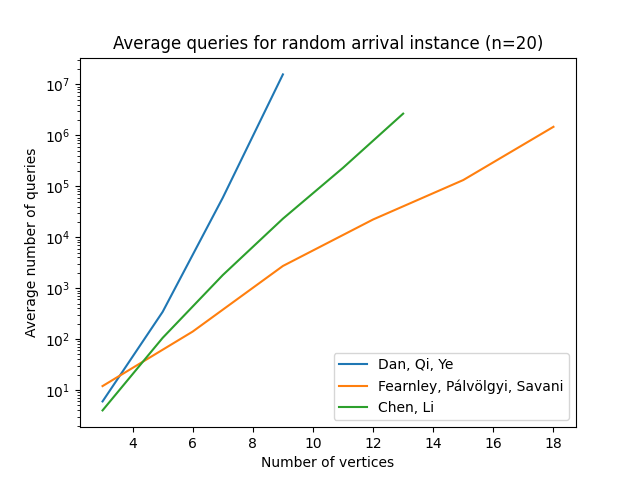
\includegraphics[width=2.6in]{plots/arrival_queries.png}
      \centering
      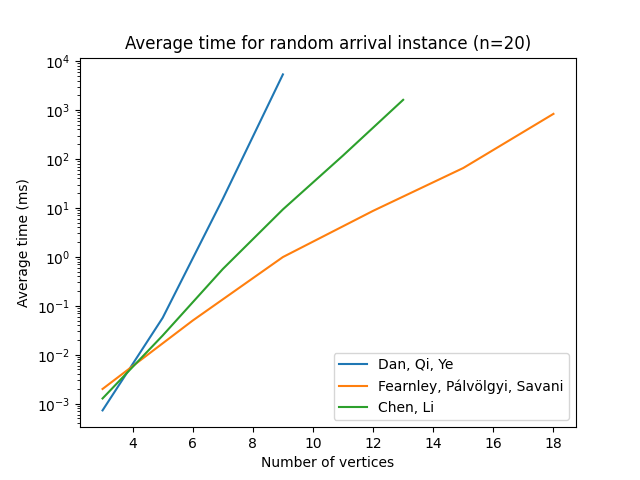
\includegraphics[width=2.6in]{plots/arrival_time.png}
      \caption{\cref{arrMainTest}} \label{arrivalMainPlot}
  \end{figure}
  \vspace{-22pt}
  \begin{figure}[H]
      \centering
      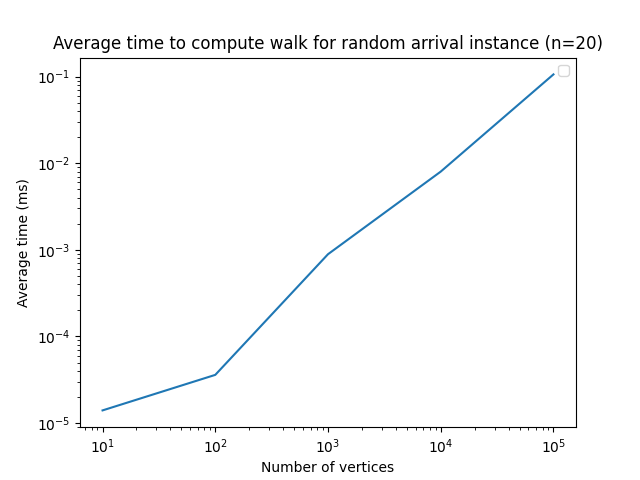
\includegraphics[width=2.6in]{plots/arrival_steps.png}
      \centering
      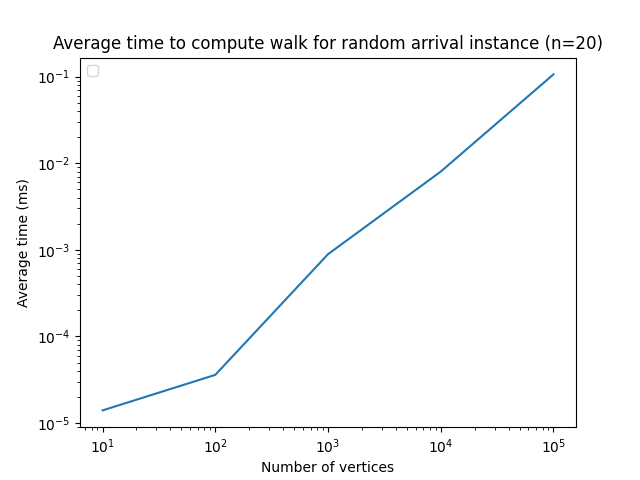
\includegraphics[width=2.6in]{plots/arrival_wtime.png}
      \caption{\cref{arrWalkTest}} \label{arrivalWalkPlot}
  \end{figure}
  \vspace{-22pt}
  \begin{figure}[H]
      \centering
      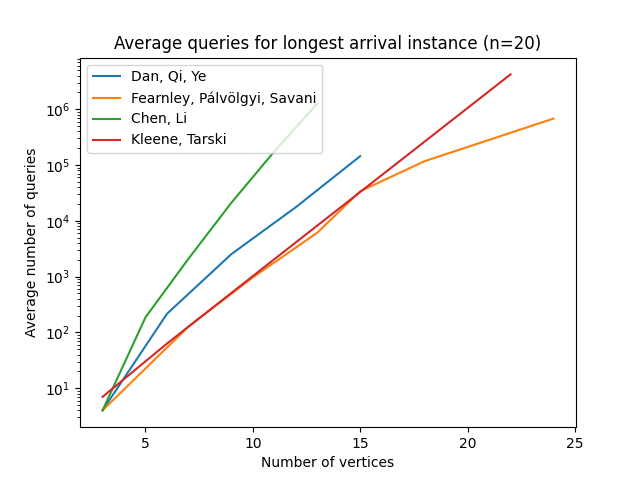
\includegraphics[width=2.6in]{plots/arrival_long_queries.png}
      \centering
      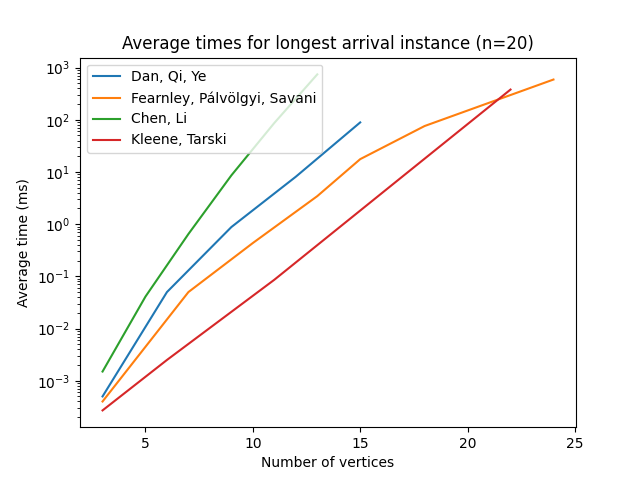
\includegraphics[width=2.6in]{plots/arrival_long_time.png}
      \caption{\cref{longArrivalTest}} \label{arrivalLongPlot}
  \end{figure}
  \vspace{-22pt}
  \begin{figure}[H] 
      \centering
      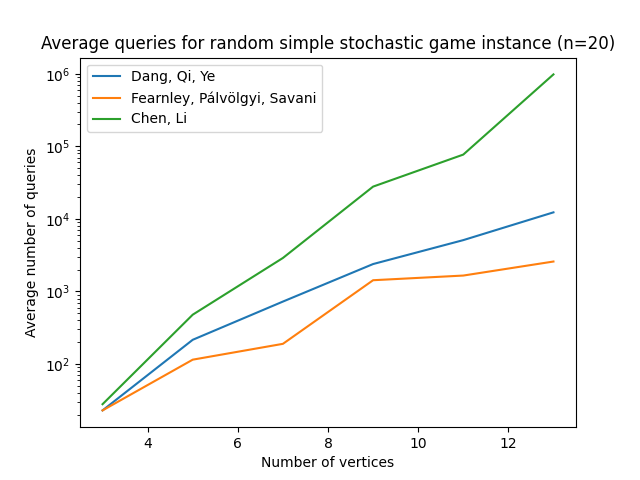
\includegraphics[width=2.6in]{plots/simple_queries.png}
      \centering
      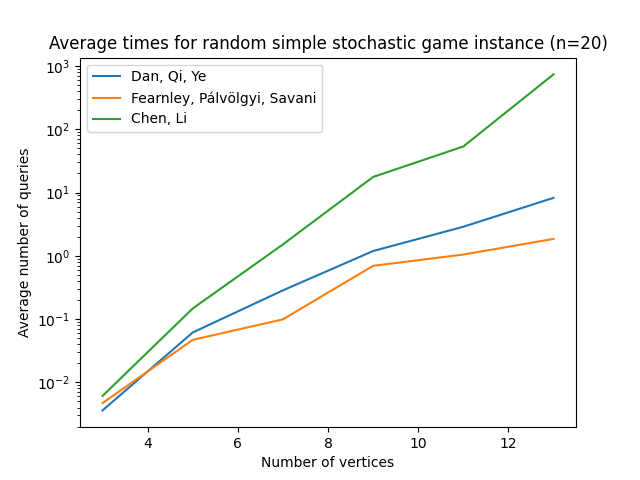
\includegraphics[width=2.6in]{plots/simple_time.png}
      \caption{\cref{ssgMainTest}} \label{simpleMainPlot}
  \end{figure}
  \vspace{-20pt}
  \begin{figure}[H]
      \centering
      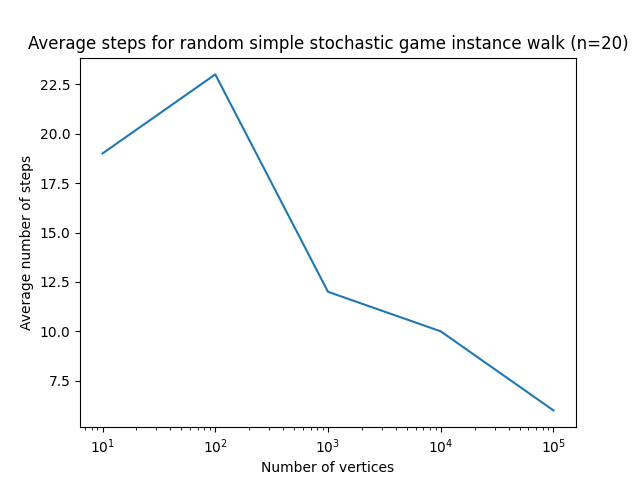
\includegraphics[width=2.6in]{plots/simple_steps.png}
      \centering
      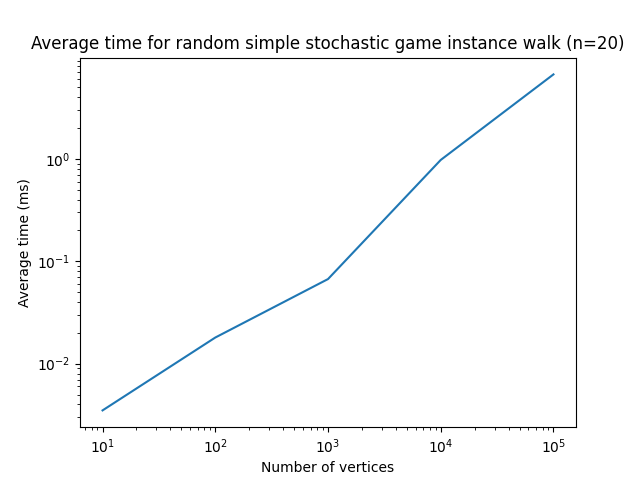
\includegraphics[width=2.6in]{plots/simple_wtime.png}
      \caption{\cref{ssgMainTest} cont.} \label{simpleWalkPlot}
  \end{figure}
  \vspace{-20pt}
  \begin{figure}[H]
      \centering
      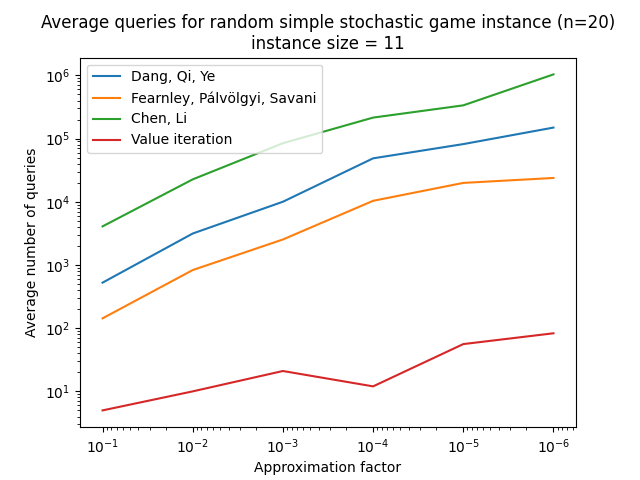
\includegraphics[width=2.6in]{plots/simple_eps_queries.png}
      \centering
      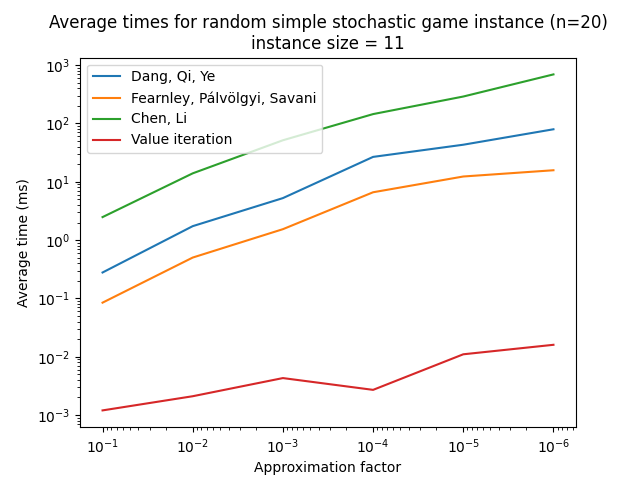
\includegraphics[width=2.6in]{plots/simple_eps_times.png}
      \caption{\cref{ssgApproxTest}} \label{simpleApproxPlot}
  \end{figure}
  \vspace{-20pt}
  \begin{figure}[H]
      \centering
      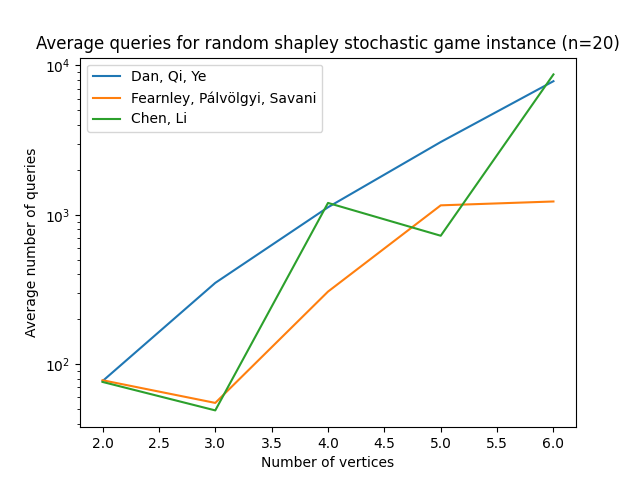
\includegraphics[width=2.6in]{plots/shapley_queries.png}
      \centering
      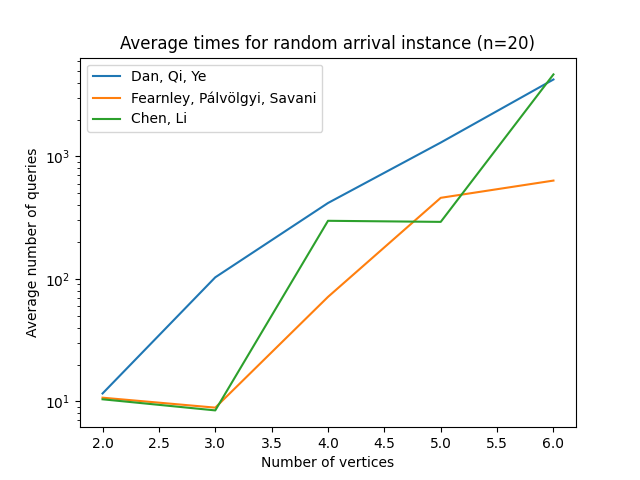
\includegraphics[width=2.6in]{plots/shapley_time.png}
      \caption{\cref{shapleyMainTest}} \label{shapleyMainPlot}
  \end{figure}
  \vspace{-20pt}
  \begin{figure}[H]
      \centering
      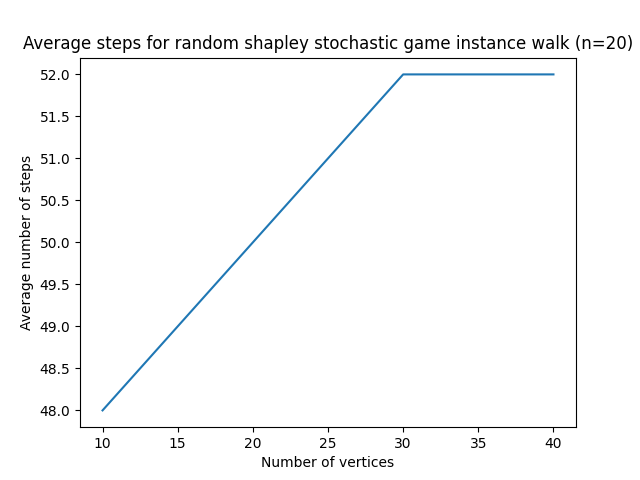
\includegraphics[width=2.6in]{plots/shapley_steps.png}
      \centering
      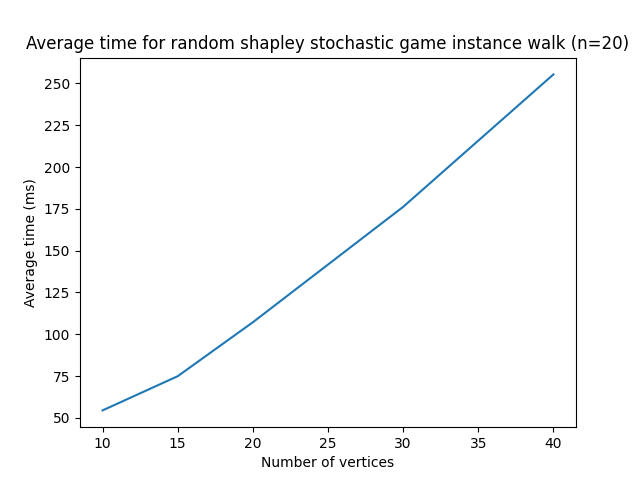
\includegraphics[width=2.6in]{plots/shapley_wtime.png}
      \caption{\cref{shapleyMainTest} cont.} \label{shapleyWalkPlot}
  \end{figure}
  \vspace{-20pt}
  \begin{figure}[H]
      \centering
      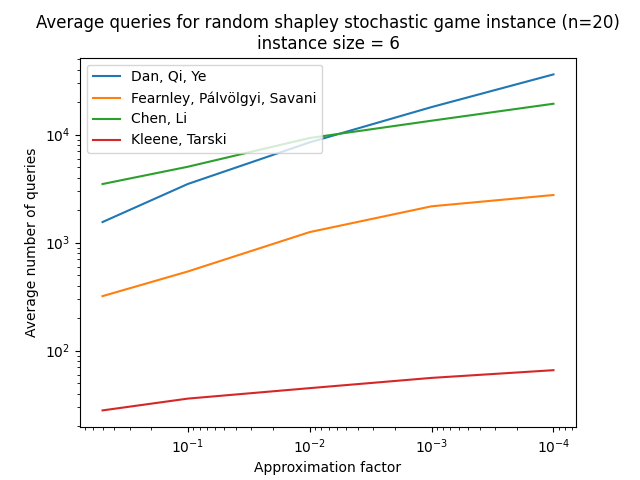
\includegraphics[width=2.6in]{plots/shapley_eps_queries.png}
      \centering
      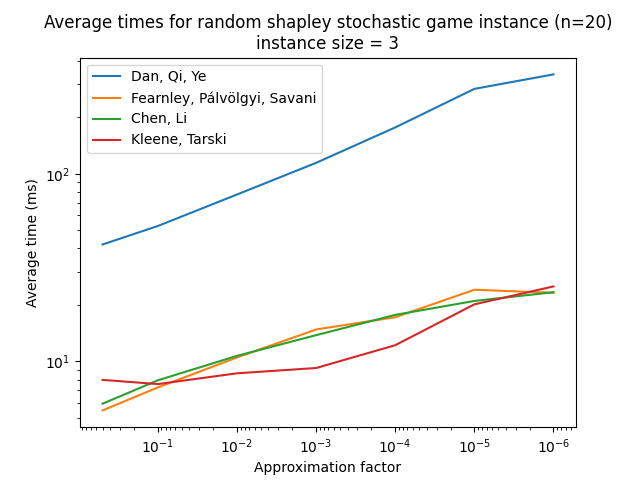
\includegraphics[width=2.6in]{plots/shapley_eps_times.png}
      \caption{\cref{shapleyApproxTest}} \label{shapleyApproxPlot}
  \end{figure}

%todo maybe add more to specific discussion sections relating
% asymptotic bounds
\section{Discussion}
On the whole, value iteration and simulating the $\arr$ walk tend to be
the most performant algorithms. Interestingly, FPS tends to be the most
performant of the binary search style algorithms, beating out the asymptotically
superior CL in almost all cases. More detailed discussion is given for individual cases below.
\subsection{$\arr$}
It can clearly be seen in \cref{arrivalMainPlot} and \cref{arrivalWalkPlot}
that simulating the arrival walk vastly outperforms the binary-search based
algorithms on randomly generated instances of the arrival problem.
The distinction is less clear when testing with the worst case instance
for the walk as seen in \cref{arrivalLongPlot}; FPS outperforms the walk
in terms of query count for more than 15 vertices, and in terms of time for more than
20. This is somewhat unexpected as the number of steps in the walk on
the worst case instance is $\Theta(2^n)$, while the upper bound we
get from FPS when applied to the walk is 
$O(\log^{\lceil (n + 2)/3 \rceil } (2^n)) = O(n^{\lceil (n + 2)/3 \rceil})$,
which is clearly a weaker bound than $O(2^n)$. I believe the cause of this
is that the recursive binary search algorithms work particularly well
on this specific long walk instance; the fixpoint for this specific instance
will be something like $\vec{x} = (2^{n}, 2^{n - 1}, ..., 1)$, and the
binary search algorithms always start by querying midpoints which happen
to be powers of two so coincide exactly with the actual fixpoint.
This perhaps motivates further testing- are there other instances
for which FPS outperforms the walk?  \\
In comparing the binary search style algorithms, it can be seen that
FPS performs best in all cases, and in particular performs better
than the asymptotically superior CL algorithm. The difference between
CL and DQY is less clear however; for random instances CL performs
better as seen in \cref{arrivalMainPlot},
but DQY performs better on the long walk instance as seen in \cref{arrivalLongPlot}.

\subsection{Simple Stochastic Games}
Similarly to $\arr$, value iteration is the most performant algorithm for solving
random simple stochastic games - it even seems to be the case
that the number of queries goes \emph{down} as the number of vertices
goes up for the walk as seen in \cref{simpleWalkPlot}. 
I believe that this is a limitation of the method
of random instance generation which perhaps motivates further investigation
into methods for generating 'hard' simple stochastic games. It could also
be the case that testing with a fixed approximiation factor $\varepsilon$
and stopping probability $\beta$ causes this behaviour. \\
In comparing the binary search based algorithms, it can be seen in \cref{simpleMainPlot} 
that
FPS is again the most performant, and DQY is the least performant. The difference
between FPS and CL is small in this case however. \\
In the test with varying approximation factor as seen in \cref{simpleApproxPlot}, value iteration 
is again the most performant, with FPS the best of the binary search algorithms.
DQY is again the slowest, with CL in the middle. Varying the approximation factor
for the simple stochastic game problem has the effect of changing the height of the lattice
that is searched; if $\beta$ is the stopping probability, and $\varepsilon$ is the approximation
factor, the associated discretized function is 
defined on $\left[\left \lfloor \frac{1}{\beta \varepsilon}\right \rfloor\right]^d$.
Since KT runs in worst case complexity $O(Nd)$ where $N$ is the height of the lattice,
and FPS in $O(\log^{\lceil \frac{2n + 2}{3} \rceil} N)$, one might expect that for
very small approximation factors that FPS is more performant. This is not shown in
the results however, so perhaps more investigation should be done into finding
instances of simple stochastic games which are 'hard' for value iteration.

\subsection{Shapley's Stochastic Games}
Testing on shapley's stochastic games was much more limited than the other two problems
as the associated monotone function took a lot longer to compute. It could be the case
the the LP solver that I used (\lstinline{soplex}\citep{soplex}) is not optimized for solving
many thousands of small LPs, or that solving LPs in this fashion will necessarily
take significantly more time than the functions for $\arr$ and simple stochastic games. \\
In comparing the algorithms running on random instances, it can be seen in \cref{shapleyMainPlot}
and \cref{shapleyWalkPlot} that 
again value iteration is the most performant. DQY is the least performant on random instances, and the difference
between CL and FPS is small. Interestingly, there seems to be some association between
the parity of the dimension and the performance of CL and FPS. I believe this is because of the
$\lceil \cdot \rceil$ in the exponent of their complexities caused by
subproblems with dimension less than 3 during decomposition, and the only reason
we don't see this in other plots is because we are measuring with less granularity on size.
Perhaps this motivates testing with more datapoints on the other problems as well. \\
The test with varying approximation factor as seen in \cref{shapleyApproxPlot} shows
again that value iteration is the most performant, and FPS is the most performant of the binary search algorithms.
There is not much difference between CL and DQY in this case. Similarly to simple stochastic games,
one would expect that for very small approximation factors that the binary search algorithms
perform better than value iteration - but again this is not seen in the results for these tests. This is again
perhaps motivation for more investigation in finding 'hard' stochastic games for the value iteration algorithm. \\
In shapley's stochastic games, many parameters were also unchanged through all tests. The maximum value
in the payoff matrix for shapley's could be varied, the stopping probabilities for both,
the number of actions at each state in shapley's, and the number of successors for all states in both
problems could all be varied. 




\chapter{Your next chapter}

A dissertation usually contains several chapters.

\chapter{Conclusions}

\section{Final Reminder}

The body of your dissertation, before the references and any appendices,
\emph{must} finish by page~40. The introduction, after preliminary material,
should have started on page~1.

You may not change the dissertation format (e.g., reduce the font size, change
the margins, or reduce the line spacing from the default single spacing). Be
careful if you copy-paste packages into your document preamble from elsewhere.
Some \LaTeX{} packages, such as \texttt{fullpage} or \texttt{savetrees}, change
the margins of your document. Do not include them!

Over-length or incorrectly-formatted dissertations will not be accepted and you
would have to modify your dissertation and resubmit. You cannot assume we will
check your submission before the final deadline and if it requires resubmission
after the deadline to conform to the page and style requirements you will be
subject to the usual late penalties based on your final submission time.

% \bibliographystyle{plain}
\bibliographystyle{plainnat}
\bibliography{mybibfile}


% You may delete everything from \appendix up to \end{document} if you don't need it.
\appendix

\chapter{First appendix}

\section{First section}

Any appendices, including any required ethics information, should be included
after the references.

Markers do not have to consider appendices. Make sure that your contributions
are made clear in the main body of the dissertation (within the page limit).

\chapter{Participants' information sheet}

If you had human participants, include key information that they were given in
an appendix, and point to it from the ethics declaration.

\chapter{Participants' consent form}

If you had human participants, include information about how consent was
gathered in an appendix, and point to it from the ethics declaration.
This information is often a copy of a consent form.


\end{document}
